\section{Parciální derivace}

\subsection{Výpočet pomocí vzorců}

Vypočtěte následující parciální derivace

\newcommand\pd[2][x]{\frac{\partial }{\partial #1}\left(\vphantom {\frac 22}#2\right)}
\begin{multicols}2
\begin{enumerate}[a)]
\item $\pd{x^2y+2xy^3+x+1}$
\item $\pd[y]{x^2y+2xy^3+x+1}$
\item $\pd{3x(3-x-2y)}$
\item $\pd[y]{3x(3-x-2y)}$
\item $\pd[x]{\sqrt{1-x^2-y^2}}$
\item $\pd[y]{\sqrt{1-x^2-y^2}}$
\item $\pd[x]{\frac x{x^2+y^2}}$
\item $\pd[y]{\frac x{x^2+y^2}}$
\end{enumerate}
\end{multicols}

\reseni
\begin{enumerate}[a)]
\item $\pd{x^2y+2xy^3+x+1}=2x\cdot y+2y^3+1+0=2xy+2y^3+1$
\item $\pd[y]{x^2y+2xy^3+x+1}=x^2+2x\cdot 3y^2+0+0=x^2+6xy$
\item $\pd{3x(3-x-2y)}=\pd{9x-3x^2-6xy}=9-3\cdot 2x-6\cdot 1\cdot y=9-6x-6y$
\item $\pd[y]{3x(3-x-2y)}=\pd[y]{9x-3x^2-6xy}=0-0-6x=-6x$
\item $\cdots=\pd[x]{(1-x^2-y^2)^{\frac 12}}=\frac 12 (1-x^2-y^2)^{-\frac 12} (0-2x-0)=
  \frac {x}{\sqrt{1-x^2-y^2}}$
\item $\cdots=\pd[y]{\sqrt{1-x^2-y^2}}= \frac {y}{\sqrt{1-x^2-y^2}}$ (z předchozího výpočtu a symetrie)
  
\item $\pd[x]{\frac x{x^2+y^2}}=\frac{1(x^2+y^2)-x(2x+0)}{(x^2+y^2)^2}=\cdots$ (derivace podílu)
\item $\pd[y]{\frac x{x^2+y^2}}=\pd[y]{x(x^2+y^2)^{-1}}=x(-1)(x^2+y^2)^{-2}(0+2y)=\cdots$ (derivace konstantního násobku mocninné funkce s vnitřní složkou)

\end{enumerate}


\konec


\obrazek{blizzard.jpg}

\subsection{Parciální derivace, pocitová teplota analyticky}
\shorthandoff{-}

Kanadský empirický vzorec pro pocitovou teplotu v zimě (wind chill factor) je
$$
%\begin{dmath*}
\begin{aligned}
W(T,v) = &13.12+0.6215 T-11.37 v^{0.16}\\&+0.3965 T v^{0.16},
\end{aligned}
%\end{dmath*}
$$
kde $T$ je teplota
(ve stupních Celsia) a $v$ je rychlost větru (v km/hod). Teplota je $-11.0\,{}^\circ\!\text{C}$  a rychlost větru $26
\,\text{km/hod}$. Určete parciální derivace pocitové teploty podle skutečné teploty a podle rychlosti větru (včetně jednotky) a výsledky interpretujte slovně.

\reseni

Dosazením do vzorce dostáváme $W(-11,26)=-20.212\,{}^\circ\!\text{C}$. Derivováním dostáváme
$$\begin{aligned}\frac{\partial W}{\partial T}(T,v)&=0.6215+0.3965 v^{0.16},\\
\frac{\partial W}{\partial v}(T,v)&=-11.37\times 0.16 v^{-0.84}+0.3965 \times 0.16 Tv^{-0.84}
\end{aligned}
$$
a po dosazení
$$\begin{aligned}\frac{\partial W}{\partial T}(-11,26)&=1.289,\\
\frac{\partial W}{\partial v}(-11,26)&=-0.163 \,{}^\circ\!\text{C}\, /(\mathrm{km}\, \text{hod}^{-1})=-0.163 \,{}^\circ\!\text{C}\, \text{hod} \,\mathrm{km}^{-1}.
\end{aligned}
$$
Za dané teploty a rychlosti větru je pocitová teplota $-20.2$ stupňů
Celsia. Nárůst teploty o jeden stupeň způsobí nárůst pocitové teploty
přibližně o $1.3$ stupně. Tedy změna teploty se projeví na pocitové
teplotě $1.3$-násobkem, tj. každkouzměnu vnímáme o třicet procent
intenzivněji.

Podobně, zesílení větru o jeden kilometr za hodinu způsobí snížení
pocitové teploty přibližně o $0.16$ stupně.

\konec

\subsection{Pocitová teplota numericky}

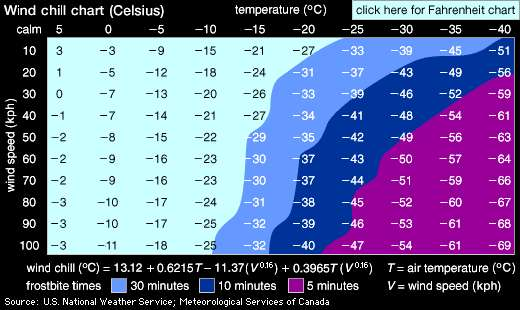
\includegraphics[width=\linewidth]{air-temperature.jpg}

\begin{enumerate}[a)]
\item Vypočtěte pomocí centrální diference parciální derivaci
$\frac {\partial W}{\partial v}$ pro teplotu $-15^\circ\mathrm C$ a rychlost větru $40\,\mathrm{km}\,\mathrm{hod}^{-1}$ a intepretujte výsledek slovně.
\item Pocitová teplota $W$ je lineární v proměnné $T$. Proto derivace $\frac{\partial W}{\partial T}$ nezávisí na $T$. Jak se tato skutečnost
  odrazí v tabulce?
  \item Odhadněte z tabulky, zda vliv větru klesá nebo roste s rychlostí větru. Potvrďte svou hypotézu analytickým výpočtem parciální derivace $\frac{\partial W}{\partial v}$ a vysvětlete fyzikálně.
\end{enumerate}

\reseni
\begin{enumerate}[a)]
\item
  $$\frac {\partial W}{\partial v}(T=-15,v=40)\approx\frac{-29-(-26)}{50-30}\frac{{}^\circ \mathrm C}{\mathrm{km}\,\mathrm{hod}^{-1}}=-0.15^\circ \mathrm C/(\mathrm{km}\,\mathrm{hod}^{-1})$$
  Za podmínek, kde je $15$ stupňů pod nulou a vítr o rychlosti $40$
kilometrů za hodinu každé další zesílení větru o kilometr za hodinu
sníží pocitovou teplotu přibližně o patnáct setin stupně.
\item Neformálně: V rámci každého řádku jsou stejně velké
  skoky. Přesněji: V každém řádku je přibližně aritmetická
  posloupnost, data se mění odečtením pevné konstantny. Případné
  fluktuace od tohoto pravidla jsou způsobeny zaokrouhlením.
\item Pokud se díváme na data po sloupcích, s rostoucí silou větru
  jsou skoky menší a proto parciálni derivace podle větru s rostoucí
  rychlostí větru klesá. To potvrzuje i analytický výpočet, protože u
  rychlosti je mocnina menší než jedna a ta se po zderivání změní na
  zápornou mocninu a tím se změní charakter závislosti na rychlosti
  větru. Fyzikálně vítr odfoukává izolační mikrovrstvu vzduchu kolem
  tváře nebo těla a proto cítíme ve větším větru větší chlad. Pokud je
  vítr silný, nestačí se tato mikrovstva vytvořit ani v minimální míře
  a proto je jedno, jestli fouká hodně nebo ještě více.
\end{enumerate}
\konec

\obrazek[Wood handbook]{wood_heat_capacity.png}
\subsection{Parciální derivace, tepelná kapacita dřeva}

Vypočtěte a slovně interpretujte parciální derivaci měrné tepelné kapacity dřeva $c$ podle teploty $T$ a podle obsahu vody MC $w$ v bodě o hodnotě MC 12\% a teplotě $27^\circ\mathrm C$.

Pro obě derivace použijte dopřednou diferenci (v tabulce nejsou ekvidistatní kroky MC).

\textit{Poznámka:} Kromě dopředné diference je možné uvažovat ještě zpětou diferenci definovanou vztahem $$\frac{f(x)-f(x-h)}{h},$$ což je vlastně dopředná diference na předhozím intervalu. Ukažte, že centrální diference je průměrem dopředné a zpětné diference.

\reseni

$$\pdv{c}{T}=\frac{1.8-1.7}{47-27}=0.005 \,\mathrm{kJ}\,\mathrm{kg}^{-1}\mathrm{K}^{-2}=5 \,\mathrm{J}\,\mathrm{kg}^{-1}\mathrm{K}^{-2}$$
Tato hodnota udává, o kolik vzroste měrná tepelná kapacita dřeva dané teploty a vlhkosti při zvýšení teploty o jeden stupeň Celsia (o jeden Kelvin).

$$\pdv{c}{w}=\frac{1.9-1.7}{20-12}=0.025 \,\mathrm{kJ}\,\mathrm{kg}^{-1}\mathrm{K}^{-1}(\text{procento MC})^{-1}=25 \,\mathrm{J}\,\mathrm{kg}^{-1}\mathrm{K}^{-1}(\text{procento MC})^{-1}$$
Tato hodnota udává, o kolik vzroste měrná tepelná kapacita dřeva dané teploty a vlhkosti při zvýšení obsahu vody o jedno procento.



Průměr centrální a zpětné diference:
\begin{dmath*}
  \frac{\frac{f(x)-f(x-h)}{h} + \frac{f(x+h)-f(x)}{h}}{2}=
  \frac{\frac{f(x)-f(x-h)+f(x+h)-f(x)}{h}}{2}=
\frac{f(x+h)-f(x-h)}{2h}
\end{dmath*}

\konec

\stranka
\subsection{Veličiny z rovnice vedení tepla}

\begin{multicols}2
V případech, kdy je při tepelné výměně nutno uvažovat vedení tepla (vysoké Biotovo číslo), modelujeme změnu teploty podle rovnice vedení tepla, kterou jsme na přednášce odvodili pro jednorozměrný případ ve tvaru
$$\varrho c \frac{\partial T}{\partial t}=\frac{\partial}{\partial x}\Bigl(\lambda\frac{\partial T}{\partial x}\Bigr).$$  Typickým případem vedení tepla v jedné dimenzi je vedení tepla ve stěně. 

Uvažujme jednorozměrnou úlohu s vedením tepla. Osa $x$ směřuje doprava, teplota v~bodě $x$ a čase $t$ je $T(x,t)$ ve stupních Celsia. Tok tepla v čase $t$ a v bodě $x$ je $q(x,t)$ v~joulech za sekundu. Kladný tok je ve směru osy $x$.
Podle Fourierova zákona je $$q=-\lambda \frac{\partial T}{\partial x}.$$

Tyč má teplotu $0\,^{\circ}\mathrm{C}$, pravý konec udržujeme na této teplotě, levý konec ohříváme na $20\,^{\circ}\mathrm{C}$ a udržujeme na této teplotě. Ve zbytku tyče (stěny) se postupně nastolí rovnováha vlivem vedení tepla.

\vspace*{-5pt}
Vyjádřete následující veličiny a určete jejich znaménko.

\vspace*{-15pt}
\begin{enumerate}[a)]\itemsep -2 pt
\item Rychlost, s jakou v daném místě a čase roste teplota jako funkce času.
\item Rychlost, s jakou v daném místě a čase roste teplota jako funkce polohy, tj. jak rychle  roste teplota směrem doprava.
\item Rychlost, jak rychle se klesá teplota jako funkce polohy, tj. směrem doprava.
\item Rychlost, se kterou roste (směrem doprava) tok tepla jako funkce polohy.
\item Rychlost, se kterou klesá (směrem doprava) tok tepla jako funkce polohy.
\end{enumerate}
\end{multicols}

\reseni
\begin{enumerate}[a)]
\item Rychlost, s jakou v daném místě a čase roste teplota jako funkce času je $\frac {\partial T}{\partial t}$ a tato derivace je v každém bodě kladná, protože tyč se ohřívá. Po čase se asi ustálí rovnováha a derivace bude nulová, teplota se přestaně měnit. Měříme ve stupních celsia za sekundu.
  $\left[\frac {\partial T}{\partial t}\right]={}^\circ\mathrm{C}\,\mathrm{s}^{-1}$
\item Rychlost, s jakou v daném místě a čase roste teplota jako funkce polohy, tj. jak rychle se roste teplota směrem doprava, je $\frac {\partial T}{\partial x}$ a tato derivace je záporná, protože vlevo je horký konec a teplota směrem doprava klesá. Měříme ve stupních celsia na metr.
    $\left[\frac {\partial T}{\partial x}\right]={}^\circ\mathrm{C}\,\mathrm{m}^{-1}$
  \item Rychlost, jak rychle se klesá teplota jako funkce polohy, tj. směrem doprava, je $-\frac {\partial T}{\partial x}$ a tato veličina je kladná, protože vlevo je horký konec a teplota směrem doprava opravdu klesá. Měříme ve stupních celsia na metr.
        $\left[-\frac {\partial T}{\partial x}\right]={}^\circ\mathrm{C}\,\mathrm{m}^{-1}$

\item Rychlost, se kterou roste (směrem doprava) tok tepla jako funkce polohy je $\frac {\partial q}{\partial x}$. Teplo teče doprava a přitom se spotřebovává, protože se ohřívá tyč. Proto tok klesá a parciální derivace je záporná.
  Měříme v joulech za sekundu na metr.
          $\left[\frac {\partial q}{\partial x}\right]=\mathrm{J}\,\mathrm{s}^{-1}\,\mathrm{m}^{-1}$
\item Rychlost, se kterou klesá (směrem doprava) tok tepla jako funkce polohy je $-\frac {\partial q}{\partial x}$ a tato veličina je kladná, což plyne z předchozího bodu a z toho, že jsme změnili znaménko.
  Měříme v joulech za sekundu na metr.
            $\left[-\frac {\partial q}{\partial x}\right]=\mathrm{J}\,\mathrm{s}^{-1}\,\mathrm{m}^{-1}$ Tato veličina udává, kolik tepla se za jednotku času ubude v toku na metrovém úseku tyče. Ze zákona zachování energie se toto teplo nemůže ``ztratit'', ale použije se na zvýšení teploty, což je vyjádřeno právě v rovnici vedení tepla.
\end{enumerate}

\konec




%\obrazek{stena_cihly}
\subsection{Okrajové podmínky pro rovnici vedení tepla}

\begin{multicols}2
  K modelu stěny pomocí rovnice vedení tepla je ještě nutné přidat podmínky související s počátečním stavem (počáteční podmínky) a s~chováním na okrajích (okrajové podmínky).

  Nechť stěna je na intervalu $x\in[0,L]$, $x=0$ je vnitřní okraj a $x=L$ je vnější okraj. Výraz $-k\frac{\partial T}{\partial x}$ udává tok tepla ve směru osy $x$. Tok ve směru osy $x$ má kladné znaménko. Naformulujte okrajové podmínky v následujících scénářích.
\begin{enumerate}[a)]\itemsep 0 pt
\item Z venku dokonale izolovaná stěna. Na hranici $x=L$ nedochází k toku tepla.
\item Vnitřní část stěny je udržovaná na konstantní teplotě $T=23^\circ \mathrm C$.
\item Stěna je zvenku osvětlená a zahřívaná Sluncem. Na vnější hranici je konstantní tok tepla směrem do stěny.
\item Stěna je zvenku ochlazována prouděním vzduchu. Tok tepla mezi stěnou a okolím je úměrný rozdílu teplot stěny a okolí.
% \item Stěna je zevnitř zahřívaná infrazářičem. Na vnitřní straně stěny je konstantní tok tepla směrem do stěny.
\item Stěna je zevnitř ohřívána prouděním vzduchu od radiátorů. Tok tepla mezi stěnou a okolím je úměrný rozdílu teplot stěny a okolí.
\end{enumerate}
\textit{Zpracováno podle Cengel: Mass and heat transfer.} 
\end{multicols}

\reseni

\begin{enumerate}[a)]
\item $\frac{\partial T}{\partial x}(L)=0$
\item $T(0)=23$
\item $-k\frac{\partial T}{\partial x}(L)=-Q$, kde $Q$ je teplo za jednotku času dodané ze Slunce. Jedná se výkon Slunce dopadající na stěnu vynásobený koeficientem absorbce, protože část tepelného výkonu se odráží. Záporné znaménko je proto, že teplo teče do stěny, tj. proti směru osy $x$.
\item $-k\frac{\partial T}{\partial x}(L)=h(T-T_{\text{okolí}})$, kde $h$ je koeficient přestupu tepla.
% \item $-k\frac{\partial T}{\partial x}(L)=Q$, kde $Q$ je teplo za jednotku času dodané z infrazářiče. Jedná se výkon dopadající na stěnu vynásobený koeficientem absorbce. Teplo teče do stěny, tj. ve směru osy $x$.
\item $-k\frac{\partial T}{\partial x}(0)=h(T_{\text{místnost}}-T)$, kde $h$ je koeficient přestupu tepla.
  Všimněte si, že poslední dvě podmínky se liší znaménkem u veličiny $T$. To proto, že v jednom případě je kladný směr toku tepla do materiálu a jednou z materiálu. Pokud chceme mít popis jednotný, nebo nezávislý na zvolené souřadné soustavě, formulujeme podmínky pro tok tepla ven z materiálu. Tento tok získáme tak, že tok tepla vynásobíme skalárně s jednotkovým vektorem směřujícím ven z materiálu kolmo na jeho povrch. V tomto případě by pro tok ze stěny do místnosti bylo $k\frac{\partial T}{\partial x}(0)=h(T-T_{\text{místnost}})$. Tento tok by byl záporný, protože ve skutečnosti teplo uniká z místnosti stěnou ven.
\end{enumerate}
\konec


\section{Gradient}

\obrazek{blizzard.jpg}

\subsection{Linearizace pocitové teploty}

Pocitová teplota $W$ z minulého cvičení má v bodě odpovídajícím teplotě $T=-11{}^\circ\mathrm C$ a rcyhlosti větru $v=26\,\mathrm {km}\,\mathrm{hod}^{-1}$ má hodnotu $$W=-20.2 ^\circ\mathrm C$$ a parciální derivace $$\pdv{W}{v}=-0.163 ^\circ\mathrm C\, \mathrm {hod}\,\mathrm{km}^{-1}$$ a
$$\pdv{W}{T}=1.289.$$ Najděte pomocí lineární aproximace vzorec pro pocitovou teplotu v okolí tohoto bodu.

\reseni

Přímým použitím vzorce pro lineární aproximaci dostáváme
\begin{dmath*}
W=-20.2+1.289(T-(-11))-0.163(v-26)=-20.2+1.289(T+11)-0.163(v-26),
\end{dmath*}
přičemž všechny veličiny dostazujeme v jednotkách SI (stupně Celsia a kilometry za hodinu).

\konec

\subsection{Parciální derivace, gradient}

Určete gradient funkcí $z=ax^2y-2xy^2$ a $h=\frac {ax}{y^2}+5x^3y^2$, kde $a\in\mathbb R$ je reálný parametr.

\reseni
\begin{align*}
  \pdv{z}{x} &= 2axy-2y^2\\
  \pdv{z}{y} &= ax^2-4xy\\
  \nabla z &= (2axy-2y^2, ax^2-4xy) = (2axy-2y^2)\vec \imath + (ax^2-4xy)\vec \jmath\\
  \pdv{h}{x} &= \frac a{y^2}+15x^2y^2\\
  \pdv{h}{y} &= ax(-2)y^{-3}+10x^3y=-\frac{2ax}{y^3}+10x^3y\\
  \nabla h &= \left(\frac a{y^2}+15x^2y^2, -\frac{2ax}{y^3}+10x^3y\right) = \left(\frac a{y^2}+15x^2y^2\right)\vec \imath + \left(-\frac{2ax}{y^3}+10x^3y\right)\vec \jmath
\end{align*}
\konec

\subsection{Gradient funkce s vrstevnicemi ve tvaru kružnic}

Určete gradient funkce $z=x^2+y^2$ a zkontrolujte, že je v každém bodě kolmý ke kružnici se středem v počátku. Využijte toho, že spojnice bodu na kružnici se středem kružnice je kolmá k této kružnici. 

\reseni
\begin{align*}
  \pdv{z}{x} &= 2x\\
  \pdv{z}{y} &= 2y\\
  \nabla z &= (2x, 2y) = 2x\vec \imath + 2y\vec \jmath
\end{align*}
Vektor $(2x,2y)$ v bodě $(x,y)$ míří směrem od počátku, tj ve směru spojnice se středem a tedy je kolmý k vrstevnici.
\konec



\subsection{Gradient funkce s paprskovitými vrstevnicemi}

Určete gradient funkce $z=\mathop{\mathrm{arctg}} \frac yx$ a zkontrolujte, že je v každém bodě tečný ke kružnici se středem v počátku. Využijte toho, že tečna je kolmá na poloměr.


\reseni
\begin{align*}
  \pdv{z}{x} &= \frac1{1+\frac {y^2}{x^2}}y\frac {(-1)}{x^2}=-\frac{y}{x^2+y^2}\\
  \pdv{z}{y} &= \frac1{1+\frac {y^2}{x^2}}\frac 1x=\frac{x}{x^2+y^2}\\
  \nabla z &=  \left(-\frac{y}{x^2+y^2},\frac{x}{x^2+y^2}\right)= \frac{1}{x^2+y^2} (-y,x)
\end{align*}
Vektor $(-y,x)$ v bodě $(x,y)$ je kolmý k vektoru $(x,y)$ a míří směrem od počátku, tj. k~poloměru. Proto je tečný ke kružnici.
\konec



\subsection{Tečná rovina atd.}

Pro funkci $f(x,y)=x^2+\frac x{y^2}-6$ najděte
\begin{enumerate}[a)]
\item gradient, 
\item gradient v bodě $(2,1)$,
\item lineární aproximaci v bodě $(2,1)$,
\item tečnou rovinu v bodě $(2,1)$,
\item rovnici vrstevnice bodem $(2,1)$ a rovnici tečny k vrstevnici tímto bodem,
\item explicitní vyjádření funkce dané v okolí bodu $(2,1)$ implicitně rovnicí $f(x,y)=0$,
\item lineární aproximace v okolí bodu $x=2$ pro funkci získanou v předchozím bodu.
\end{enumerate}

\reseni
\begin{enumerate}[a)]
\item $\nabla f=\left(2x+\frac 1{y^2},-2\frac x{y^3}\right)$
\item $\nabla f(2,1)=(5,-4)$
\item $f(x,y)\approx 5(x-2)-4(y-1)$
\item $z= 5(x-2)-4(y-1)$
\item Rovnice vrstevnice je $$x^2+\frac x{y^2}-6=0$$
  a tečna $$5(x-2)-4(y-1)=0,$$ tj. $$5x-4y-6=0.$$
\item Postupnými úpravami a výběrem správného znaménka po vyřešení kvadratické rovnice vzhledem k $y$ dostáváme
  $$
  \begin{aligned}
    x^2+\frac x{y^2}-6&=0\\
        \frac x{y^2}&=6-x^2\\
        y^2&=\frac{x}{6-x^2}\\
        y&=\sqrt{\frac{x}{6-x^2}}\\
  \end{aligned}
$$
\item Z rovnice tečny k vrstevnici $$5(x-2)-4(y-1)=0$$
  dostáváme $$y=1+\frac 54 (x-2)$$
  a proto
  $$\sqrt{\frac{x}{6-x^2}}\approx 1+\frac 54 (x-2)$$ v okolí $x=2$.
\end{enumerate}

\konec


\subsection{Linearizace vektorové funkce, Jacobiho matice}

Jacobiho matice se používá k linearizaci vektorových funkcí, které
mají na vstupu i na výstupu vektor. Jsou to matice, kde gradienty
jednotlivých komponent vektorové funkce jsou zapsány do řádků matice.

Najděte Jacobiho matici pro funkci $$\vec F(x,y)=(x^2+xy+6y)\vec i + e^{3x}\vec j$$ a poté hodnotu této matice v bodě $(0,0)$.

\reseni

Platí
\begin{align*}
  \frac{\partial }{\partial x}\left(x^2 +xy+6y\right) &=2x+y\\
  \frac{\partial }{\partial y}\left(x^2 +xy+6y\right) &=x+6\\
  \frac{\partial }{\partial x}\left(e^{3x}\right) &=3e^{3x}\\
  \frac{\partial }{\partial y}\left(e^{3x}\right) &=0\\
\end{align*}
a proto má Jacobiho matice tvar
\begin{equation*}
  J(x,y)=
  \begin{pmatrix}
    2x+y & x+6\\ 3e^{3x} & 0
  \end{pmatrix}.
\end{equation*}
V bodě $(0,0)$ potom 
\begin{equation*}
  J(0,0)=
  \begin{pmatrix}
    0 & 6\\ 3 & 0
  \end{pmatrix}.
\end{equation*}


\konec


\obrazek[Wood handbook]{anatomicke_smery_dreva.png}

\subsection{Parciální derivace, gradient a násobení matic}

Vypočtěte gradient funkce $$T=10-\sqrt{x^2+y^2}.$$ Ukažte, že vrstevnice
této funkce jsou kružnice se středem v počátku, nakreslete obrázek s
těmito vrstevnicemi a vyznačte do tohoto obrázku gradienty v bodech
$A=(0,1)$, $B=(1,0)$ a $C=(1,1)$

Uvažujte součinitel tepelné vodivosti $$\lambda =
\begin{pmatrix}
  2&0\\0&3
\end{pmatrix}$$
a vypočtěte tok tepla v bodech $A$, $B$, $C$. Porovnejte směr tohoto toku se směrem gradientu a vysvětlete svá pozorování. Snaží se matice usměrnit teplo do  směru osy $x$ nebo do  směru osy $y$? Odpovídá situace spíše dřevu s podélným směrem v ose $x$ nebo v ose $y$?


\reseni

Platí $$\pdv{T}{x}=-\frac 12 (x^2+y^2)^{-\frac 12}(2x)=-\frac{x}{\sqrt{x^2+y^2}}$$
a ze symetrie 
$$\pdv{T}{y}=-\frac{y}{\sqrt{x^2+y^2}}.$$
Odsud $$\nabla T=\qty(-\frac{x}{\sqrt{x^2+y^2}},-\frac{y}{\sqrt{x^2+y^2}})^T
=
-\frac 1{\sqrt{x^2+y^2}}(x,y)^T.$$
Tok tepla je
$$\vec q=-\lambda \nabla T=\frac 1{\sqrt{x^2+y^2}}\begin{pmatrix}
  2&0\\0&3
\end{pmatrix}
\begin{pmatrix}
  x\\y
\end{pmatrix}
=\frac 1{\sqrt{x^2+y^2}} \begin{pmatrix}
  2x\\3y
\end{pmatrix}
$$
Dosazením dostáváme $\vec q(A)=(0,3)^T$, $\vec q(B)=(2,0)^T$, $\vec q(C)=\frac 1{\sqrt{2}}(2,3)^T$. Porovnáním s gradientem $\nabla T(A)=-(0,1)^T$, $\nabla T(B)=-(1,0)^T$ a $\nabla T(C)=-\frac 1{\sqrt 2}(1,1)^T$ vidíme, že v bodech $A$  a $B$ je tok proti směru gradientu, v bodě $C$ se tok stáčí do směru osy $y$. Protože ve ose $y$ má dřevo větší vodivost, jedná se o podélný směr. To je ale vlastně vidět už ze zadané matice.

\konec


\stranka
\section{Divergence, rovnice vedení tepla}


\subsection{Divegrence vektorového pole}

\begin{enumerate}[a)]
\item Vypočtěte divergenci vektorového pole
  $$\vec F=x^2y\vec \imath + (x+y^2)\vec \jmath.$$
\item Zakreslete do obrázku směr toku vektorového pole v bodě $(2,1)$. 
\item Vypočtěte divergenci vektorového pole v bodě $(2,1)$ a podle toho, zda je kladná nebo záporná rozhodněte, zda se tok v daném bodě zhušťuje nebo řídne.
\item Předpokládejme, že dané vektorové pole reprezentuje stacionární tok. Je v bodě $(2,1)$ zdroj nebo spotřebič?
\end{enumerate}
\reseni

\begin{enumerate}[a)]
\item $\nabla \cdot \vec F=\pdv{x}(x^2y)+\pdv{y}(x+y^2)
=2xy+(0+2y)=2y(x+1)$
\item $\vec F(2,1)=2^2\cdot 1\vec \cdot \imath + (2+1^2)\vec \jmath=4\vec\imath+3\vec\jmath=(4,3)$, tj. vektorové pole teče směrem doprava nahoru směrem daným směrnicí $0.75$, tj. pod úhlem menším než $45^\circ$.
\item $\nabla\cdot\vec F(2,1)=2\cdot 1 \cdot(2+1)=6>0$. Divergence je kladná a proto se tok zahušťuje.
\item Zdroj (kladná divergence).
\end{enumerate}
\konec

\subsection{Divegrence vektorového pole s parametrem}

\begin{enumerate}[a)]
\item Vypočtěte divergenci vektorového pole
  $$\vec F=ax^3y^2\vec \imath + 3x^2y\vec \jmath,$$ kde
  $a\in\mathbb R$ je reálný parametr.
\item Určete hodnotu parametru $a$ tak, aby pole bylo v bodě $(-1,2)$ nezřídlové, tj. aby mělo nulovou divergenci v bodě $(-1,2)$.
\end{enumerate}
\reseni

\begin{enumerate}[a)]
\item $\nabla \cdot \vec F=\pdv{x}(ax^3y^2)+\pdv{y}(3x^2y)
=3ax^2y^2+3x^2=3x^2(ay^2+1)$
\item $\nabla \cdot \vec F (-1,2)=3(-1)^2(a\cdot 2^2+1)=3(4a+1) $ a $\nabla \cdot \vec F (-1,2)=0$ pokud $3(4a+1)=0$, tj. $a=-\frac 14$.
\end{enumerate}
\konec

\obrazek{drevo_textura.jpg}

\subsection{Rovnice vedení tepla v dvourozměrném materiálu}

Teplota ve dvourozměrné desce pro $0\leq x\leq 10$ a $0\leq y\leq 10$ zachycené v určitém okamžiku termokamerou je popsána rovnicí
  $$T(x,y)=(2x-y)^2+x^4.$$
  Rozměry jsou v centimetrech, teplota ve stupních Celsia. (Formálně to nevychází, ale ke každému členu můžeme dodat konstantu, která jeho rozměr opraví. Pro jednoduchost tuto komplikaci vynecháme.)

\begin{enumerate}[a)]
\item Vypočtěte gradient $\nabla T$  a tok tepla $-k \cdot \nabla T.$
Součinitel tepelné vodivosti (v jednotkách kompatibilních se zadáním) je $k=
  \begin{pmatrix}
    4 & 1\\1&6
  \end{pmatrix}.
$ 
\item Určete, zda na levém okraji desky teče teplo dovnitř desky nebo z desky ven.
\item Vypočtěte divergenci toku tepla, tj. $\nabla\cdot(-k \cdot \nabla T).$
\item V desce nejsou zdroje tepla. Ochlazuje se deska uprostřed, nebo otepluje?
\end{enumerate}

\reseni
\begin{enumerate}[a)]
\item Gradient je vektor složený z parciálních derivací. $$\nabla T=\qty(
  4(2x-y)+4x^3,-2(2x-y))^T$$ Tok je tenzor vodivosti maticově vynásobený s gradientem teploty a faktorem $(-1)$.
  $$-k\cdot \nabla T=-
  \begin{pmatrix}
    4&1\\1&6
  \end{pmatrix}
  \begin{pmatrix}
    4(2x-y)+4x^3\\-2(2x-y)
  \end{pmatrix}
  =-
  \begin{pmatrix}
    14(2x- y)+16x^3\\-8(2x- y)+4x^3
  \end{pmatrix}
$$
\item Do vztahu pro tok dosadíme rovnici levého okraje desky, tj. $x=0$.
  $$-k\cdot \nabla T (x=0)=
  \begin{pmatrix}
    14y\\-8y
  \end{pmatrix}
  $$
  
  Na levém okraji desky je $y>0$ a proto $14y>0$. Tok míří doprava a teplo teče na tomto okraji do desky.
\item  Vypočteme divergenci toku určeného v prvním bodě. $$
  \begin{aligned}
\nabla \cdot (-k\cdot \nabla T )&=\pdv{x}(-14(2x- y)-16x^3)+\pdv{y}(8(2x- y)-4x^3)\\&=-48x^2-28-8\\&=-48x^2-36
\end{aligned}
$$
\item Do vztahu pro diveregenci dosadíme bod, který nás zajímá. $$\nabla \cdot (-k\cdot \nabla T )(x=5,y=5)=-1236$$ Tok tepla se zmenšuje a protože jde o stav bez zdrojů, teplo se v daném místě akumuluje a deska se proto otepluje. Z rovnice vedení tepla
  $$\rho c\pdv{T}{t}=\nabla\cdot(k \cdot \nabla T)$$
  plyne v daném bodě
  $$\rho c\pdv{T}{t}=1236$$
  a můžeme dokonce odhadnout, jak rychle teplota roste.
\end{enumerate}
\konec

% var('x,y')
% k=matrix([[5,1],[1,4]])
% T(x,y)=(x+2*y)^2+x^3
% show(T.gradient())
% show(-k*T.gradient())
% show(-k*T.gradient()(x=0))
% show((-k*T.gradient())[0].diff(x)+(-k*T.gradient())[1].diff(y))

\subsection{Vedení tepla v různých materiálech}

\begin{enumerate}[a)]
\item Zapište rovnici vedení tepla v trojrozměrném izotropním a v
  trojrozměrném ortotropním materiálu. Ve druhém případě volte osy ve
  směru vlastních vektorů.
\item Napište, jak je možné zjednodušit rovnice z předchozího bodu,
  pokud jsou materiálové konstanty nezávislé na poloze (homogenní
  materiál) a na teplotě (lineární materiál).
\end{enumerate}

\reseni
\begin{enumerate}[a)]
\item Izotropní: $\varrho c \pdv{T}{t} = 
\pdv{x}(k\pdv{T}{x})
+\pdv{y}(k\pdv{T}{y})
+\pdv{z}(k\pdv{T}{z})$

  Ortotropní:
 $\varrho c \pdv{T}{t} = 
\pdv{x}(k_x\pdv{T}{x})
+\pdv{y}(k_y\pdv{T}{y})
+\pdv{z}(k_z\pdv{T}{z})
$
\item Izotropní: $\varrho c \pdv{T}{t} = 
k\left(\pdv[2]{T}{x} + \pdv[2]{T}{y} + \pdv[2]{T}{z}\right)
$

  Ortotropní:
 $\varrho c \pdv{T}{t} = 
k_x\pdv[2]{T}{x}
+k_y\pdv[2]{T}{y}
+k_z\pdv[2]{T}{z}
$
\end{enumerate}
\konec

\section{Rotace, kmenová funkce gradientu}


\subsection{Rotace vektorového pole v rovině}

Vypočtěte rotaci funkce $\vec F=xy^2\vec \imath + 2xy\vec\jmath$.

\reseni

 $$
 \begin{aligned}
\curl \vec F=
 \begin{vmatrix}
   \vec\imath & \vec \jmath & \vec k\\
   \pdv{x} & \pdv{y} & \pdv{z} \\
   xy^2 & 2xy & 0
 \end{vmatrix}
 &=\vec k\qty({\pd[x]{2xy}-\pd[y]{xy^2}})\\&
 =\vec k(2y-2xy)\\&=2y(1-x)\vec k
\end{aligned}
 $$



\konec

\subsection{Rotace vektorového pole v prostoru}

Vypočtěte rotaci funkce $\vec F=xyz\vec \imath + 5x^2y\vec\jmath-3x^2z\vec k$.

\reseni

 $$
 \begin{aligned}
\curl \vec F&=
 \begin{vmatrix}
   \vec\imath & \vec \jmath & \vec k\\[4pt]
   \pdv{x} & \pdv{y} & \pdv{z} \\[10pt]
   xyz& 5x^2y & -3x^2z
 \end{vmatrix}\\
 &=
\vec \imath \ \qty[\pd[x]{-3x^2z}-\pd[z]{5x^2y}]
\\&\quad +\vec \jmath \ \qty[\pd[z]{xyz}-\pd[x]{-3x^2z}] 
\\&\quad +\vec k\ \qty({\pd[x]{5x^2y}-\pd[y]{xyz}})\\
 &=(xy+6xz)\vec\jmath + (10xy-xz)\vec k
\\&=x(y+6z)\vec\jmath + x(10y-z)\vec k
\end{aligned}
 $$



\konec

\subsection{Divergence a rotace 2D funkce s parametrem}
Vypočtěte divergenci a rotaci funkce $\vec F=ax^2y^3\vec \imath + (x^2+y)\vec\jmath$.

\reseni

$$\nabla\cdot \vec F=\pdv{x}(ax^2y^3)+\pdv{y}(x^2+y)=2axy^3+1$$

 $$\curl \vec F=
 \begin{vmatrix}
   \vec\imath & \vec \jmath & \vec k\\
   \pdv{x} & \pdv{y} & \pdv{z} \\
   ax^2y^3 & x^2+y & 0
 \end{vmatrix}
 =\vec k(2x-3ax^2y^2)
 $$

\konec


\subsection{Nalezení kmenové funkce 1/3}

Pro vektorové pole $$\frac 45 x y^3\vec \imath + \frac 65x^2y^2\vec\jmath$$ najděte funkci $\varphi$ tak, že zadané vektorové pole je rovno gradientu $\nabla \varphi.$

\reseni

Platí $\pdv {\varphi}{x}=\frac 45 xy^3$ a $\pdv{\varphi}{y}=\frac 65 x^2y^2$.

Odsud
$$\varphi =\int \pdv{\varphi}{x} \,\mathrm dx=\int \frac 45 xy^3 \,\mathrm dx
=\frac 45 \frac {x^2}{2}y^3=\frac 25 x^2y^3+C_1(y)$$
a
$$\varphi =\int \pdv{\varphi}{y} \,\mathrm dy=\int \frac 65 x^2y^2 \,\mathrm dy
=\frac 65 {x^2}\frac{y^3}3=\frac 25 x^2y^3+C_2(x).$$
Porovnáním musí být $C_1(y)=C_2(x)=C\in\mathbb R$ a
$$\varphi(x,y)=\frac 25 x^2y^3+C,\quad C\in\mathbb R.$$


\konec

\subsection{Nalezení kmenové funkce 2/3}

Pro vektorové pole $$\left(x^2+\frac 45 x y^3\right)\vec \imath + \left(\frac 65x^2y^2+y\right)\vec\jmath$$ najděte funkci $\varphi$ tak, že zadané vektorové pole je rovno gradientu $\nabla \varphi.$

\reseni

Platí $\pdv {\varphi}{x}=x^2+\frac 45 xy^3$ a $\pdv{\varphi}{y}=\frac 65 x^2y^2+y$.

Odsud
$$\varphi =\int \pdv{\varphi}{x} \,\mathrm dx=\int x^2+\frac 45 xy^3 \,\mathrm dx
=\frac {x^3}3+\frac 45 \frac {x^2}{2}y^3=\frac {x^3}3+\frac 25 x^2y^3+C_1(y)$$
a
$$\varphi =\int \pdv{\varphi}{y} \,\mathrm dy=\int \frac 65 x^2y^2 +y \,\mathrm dy
=\frac 65 {x^2}\frac{y^3}{3}+\frac 12 y^2=\frac 25 x^2y^3+\frac 12 y^2 + C_2(x).$$
Porovnáním musí být $C_1(y)=\frac 12 y^2+C$ a $C_2(x)=\frac {x^3}3+C$, $C\in\mathbb R$ a
$$\varphi(x,y)=\frac {1}{3}x^3+\frac 25 x^2y^3+\frac 12 y^2+C,\quad C\in\mathbb R.$$

\konec

\subsection{Nalezení kmenové funkce 3/3}

Pro vektorové pole $$\left(y+\frac 45 x y^3\right)\vec \imath + \left(\frac 65x^2y^2+x^2\right)\vec\jmath$$ najděte funkci $\varphi$ tak, že zadané vektorové pole je rovno gradientu $\nabla \varphi.$



\reseni

Platí $\pdv {\varphi}{x}=y+\frac 45 xy^3$ a $\pdv{\varphi}{y}=\frac 65 x^2y^2+x^2$.

Odsud
$$\varphi =\int \pdv{\varphi}{x} \,\mathrm dx=\int y+\frac 45 xy^3 \,\mathrm dx
=xy+\frac 45 \frac {x^2}{2}y^3=xy+\frac 25 x^2y^3+C_1(y)$$
a
$$\varphi =\int \pdv{\varphi}{y} \,\mathrm dy=\int \frac 65 x^2y^2 +x^2 \,\mathrm dy
=\frac 25 {x^2}\frac{y^3}3+x^2y=\frac 25 x^2y^3+x^2y+ C_2(x).$$
Porovnáním musí být
$$xy+C_1(y)=x^2y+C_2(x),$$
což není možné splnit.

Ověříme, že parciální derivace
$\pdv {y} \qty(y+\frac 45 xy^3)$ a $\pdv{x}\qty(\frac 65 x^2y^2+x^2)$ jsou různé.
Platí
$$\pdv {y} \qty(y+\frac 45 xy^3)=1+\frac{12}5xy^2$$
a
$$\pdv{x}\qty(\frac 65 x^2y^2+x^2)=\frac {12}5 xy^2+2x$$
a protože obě parciální derivace jsou různé, kmenová funkce neexistuje.

\konec

\newpage

\section{Křivkové integrály}

\nonstopmode

\subsection{Křivkový integrál druhého druhu po třech různých křivkách}


Vypočtěte $$\int_{C_i} \vec F \mathrm d\vec r$$ pro vektorové pole $$\vec F=-y\vec \imath + x\vec\jmath$$ po třech různých křivkách $C_1$, $C_2$ a $C_3$.
\begin{align*}
  C_1&\colon \vec r=\cos(t)\vec \imath + \sin (t)\vec\jmath, \quad t\in\qty[0,\frac\pi 2]\\
  C_2&\colon \vec r=(1-t)\vec \imath + t\vec\jmath, \quad t\in\qty[0,1]\\
  C_3&\colon \vec r=(1-t^2)\vec \imath + t\vec\jmath, \quad t\in\qty[0,1]
\end{align*}
Tj. počítáme
$$\int_{C_i} -y\,\mathrm dx + x\,\mathrm dy$$
po třech zadaných křivkách $C_1$, $C_2$ a $C_3$.

\reseni

Vektory budeme pro stručnost zapisovat jako uspořádané dvojice.

\stranka

\textbf{Křivka $C_1$.}
Derivací křivky $\vec r=(\cos(t),\sin(t))$ podle $t$ dostáváme
$$\frac{\mathrm d\vec r}{\mathrm dt}=(-\sin (t),\cos (t)).$$
Rovnice vektorového pole podél křivky má tvar
$$\vec F(\vec r(t))=(-\sin t,\cos t).$$
Skalárním součinem dostáváme
$$\vec F \frac{\mathrm d\vec r}{\mathrm dt}=
(-\sin t,\cos t)\cdot (-\sin (t),\cos (t)) = \sin^2 t+\cos^2 t =1.
$$
Odsud formálně $$\vec F\mathrm d\vec r=1\mathrm dt$$
a integrál má tvar
$$\int_C\vec F\mathrm d\vec r=\int_0^{\frac \pi 2}1\,\mathrm dt=\frac \pi 2,$$
kde poslední Riemannův integrál není nutné počítat, protože integrál z jedničky je délka intervalu, přes který se integruje.

\stranka

\textbf{Křivka $C_2$.}
Derivací křivky $\vec r=(1-t,t)$ podle $t$ dostáváme
$$\frac{\mathrm d\vec r}{\mathrm dt}=(-1,1).$$
Rovnice vektorového pole podél křivky má tvar
$$\vec F(\vec r(t))=(-t,1-t).$$
Skalárním součinem dostáváme
$$\vec F \frac{\mathrm d\vec r}{\mathrm dt}=
(-t,1- t)\cdot (-1,1) = (-t)(-1)+(1-t)\cdot 1 =1.
$$
Odsud formálně $$\vec F\mathrm d\vec r=1\mathrm dt$$
a integrál má tvar
$$\int_C\vec F\mathrm d\vec r=\int_0^{1}1\,\mathrm dt=1,$$
kde ani v tomto případě poslední Riemannův integrál není nutné počítat, protože integrál z jedničky je délka intervalu, přes který se integruje.

\stranka

\textbf{Křivka $C_3$.}
Derivací křivky $\vec r=(1-t^2,t)$ podle $t$ dostáváme
$$\frac{\mathrm d\vec r}{\mathrm dt}=(-2t,1).$$
Rovnice vektorového pole podél křivky má tvar
$$\vec F(\vec r(t))=(-t,1-t^2).$$
Skalárním součinem dostáváme
$$\vec F \frac{\mathrm d\vec r}{\mathrm dt}=
(-t,1- t^2)\cdot (-2t,1) = (-t)(-2t)+(1-t^2)\cdot 1 =t^2+1.
$$
Odsud formálně $$\vec F\mathrm d\vec r=(t^2+1)\mathrm dt$$
a integrál má tvar
$$\int_C\vec F\mathrm d\vec r=\int_0^{1}(t^2+1)\,\mathrm dt=
\qty[\frac 13 t^3 + t]_0^1 = \frac 13 + 1 - 0 =\frac 43.
$$

\stranka

\obrazek[vlastní]{priklad_5_1_prace.png}

\textbf{Interpretace jako práce, srovnání.}

Všechny křivky jsou z bodu $[1,0]$ do bodu $[0,1]$. Nejblíže k počátku je úsečka $C_2$, nejdále je čvrtkružnice $C_1$, křivka $C_2$ je mezi nimi.

Integrál fyzikálně znamená práci vektorového pole $(-y,x)$ po zadané křivce. Toto vektorové pole míří po kružnicích okolo počátku proti směru hodinových ručiček. Délka vektoru je rovna vzdálenosti od počátku.

Křivka $C_1$ je nejdále od počátku a vektorové pole je na ní nejsilnější. Navíc v každém bodě je síla ve směru křivky a proto se projeví ve výsledném příspěvku bez redukování. Díky tomu můžeme integrál po kružnici počítat stejně jako práci na přímce, tj. součinem délky  křivky $\frac \pi 2$ a velikosti síly $|\vec F|=1$. Po dalších křivkách je síla menší (křivky jdou blíže ke středu) a navíc se neuplatní celá velikost síly, protože síla svírá s křivkou nenulový úhel a při práci se projeví pouze tečná komponenta.


\stranka

\obrazek[vlastní]{priklad_5_1.png}

%https://sagecell.sagemath.org/?z=eJx1kMFuwjAQRO-R8g8rgRRHMW3snH3iB3LgRmgUEkMNxo5sQ5u_r01SlbbhtCPN7hvN3hqDkiFJ40hcem0cqOulH-LIEXZXL1Io2zctRzkGhXrxSlNM8twfODqzQiZzTdh222qLRIqtUH7s4KANCBAKHNn5Deo3yEpg8ejQ4BSj80b_eyVhUlhX91I7tCYYgjhpoXjHNubKMUh-5KqrZbPnkplkua5J1WqpFSA_LThc2UBLl0laxVH2gKMzuHBqWGJ4l8yx6chGZOXwHLJ4jjwaztUstPiB-h_csXHku1MWWPWNt06b-iC47BD6xEOKwY8ckyCGSUwpe9m053Bv3_UHKklW-paN7T2jNo0TmpE7PI4WZTHHHzKK8zFhRb4jJvWriccsxpCsLP5mYHDCSe77bfQZei05LCsfBCc2JfiSX8c_x8Q=&lang=sage&interacts=eJyLjgUAARUAuQ==

\textbf{Interpretace jako tok, srovnání.}

Všechny křivky jsou z bodu $[1,0]$ do bodu $[0,1]$. Nejblíže k počátku je úsečka $C_2$, nejdále je čvrtkružnice $C_1$, část paraboly $C_2$ je mezi nimi.

Integrál fyzikálně znamená tok vektorového pole $(x,y)$ křivkou. Toto vektorové pole míří směrem z počátku a zesiluje směrem od počátku, protože délka vektoru je rovna vzdálenosti od počátku.

Proto je hodnota po křivce nejblíže počátku nejmenší atd. Na křivce $C_1$ (kružnice) je tok v~každém bodě kolmý ke křivce a stejně velký a proto je celkový tok snadné určit jako součin velikosti vektorového pole na křivce ($|\vec F|=1$) a délky křivky $\frac \pi 2$.


\konec


\subsection{Křivkový integrál druhého druhu po parabole}


Vypočtěte $$\int_{C} \vec F \mathrm d\vec r$$ pro vektorové pole $$\vec F=x^2\vec \imath + (x+y)\vec\jmath$$ po části paraboly
\begin{align*}
  C&\colon \vec r=t\vec \imath + t^2\vec\jmath, \quad t\in\qty[0,1]
\end{align*}
tj. počítáme
$$\int_C x^2\,\mathrm dx + (x+y)\,\mathrm dy$$
po zadané křivce $C$.

\reseni

Vektory budeme pro stručnost zapisovat jako uspořádané dvojice.

\stranka

Derivací křivky $\vec r=(t,t^2)$ podle $t$ dostáváme
$$\frac{\mathrm d\vec r}{\mathrm dt}=(1,2t).$$
Rovnice vektorového pole podél křivky má tvar
$$\vec F(\vec r(t))=(t^2,t+t^2).$$
Skalárním součinem dostáváme
$$\vec F \frac{\mathrm d\vec r}{\mathrm dt}=
(1,2t)\cdot (t^2,t+t^2) = 1\cdot t^2+2t\cdot(t+t^2)=3t^2+2t^3.
$$
Odsud formálně $$\vec F\mathrm d\vec r=(3t^2+2t^3)\mathrm dt$$
a integrál má tvar
$$\int_C\vec F\mathrm d\vec r=\int_0^{1}(3t^2+2t^3)\,\mathrm dt
=\qty[t^3+\frac 12 t^4]_0^1=1+\frac 12 - 0 = \frac 32.$$

\konec

\stranka


\subsection{Křivkový integrál druhého druhu po kubické parabole}


Vypočtěte $$\int_{C} \vec F \mathrm d\vec r$$ pro vektorové pole $$\vec F=2y\vec \imath + x^2y\vec\jmath$$ po části kubické paraboly
\begin{align*}
  C&\colon \vec r=t\vec \imath + t^3\vec\jmath, \quad t\in\qty[0,1],
\end{align*}
tj. počítáme
$$\int_C 2y\,\mathrm dx + x^2y\,\mathrm dy$$
po zadané křivce $C$.

\reseni

Vektory budeme pro stručnost zapisovat jako uspořádané dvojice.

\stranka

Derivací křivky $\vec r=(t,t^3)$ podle $t$ dostáváme
$$\frac{\mathrm d\vec r}{\mathrm dt}=(1,3t^2).$$
Rovnice vektorového pole podél křivky má tvar
$$\vec F(\vec r(t))=(2t^3,t^2t^3)=(2t^3,t^5).$$
Skalárním součinem dostáváme
$$\vec F \frac{\mathrm d\vec r}{\mathrm dt}=
(1,3t^2)\cdot (2t^3,t^5) = 1\cdot 2t^3+3t^2\cdot t^5=2t^3+3t^7.
$$
Odsud formálně $$\vec F\mathrm d\vec r=(2t^3+3t^7)\mathrm dt$$
a integrál má tvar
$$\int_C\vec F\mathrm d\vec r=\int_0^{1}(2t^3+3t^7)\,\mathrm dt
=\qty[\frac 12 t^4 + \frac 38 t^8]_0^1=\frac 12 +\frac 38 - 0 = \frac 78.$$

\konec


\stranka


\obrazek[vlastní]{priklad_5_4.png}

\subsection{Tok vektorového pole uzavřenou křivkou}

Vypočtěte tok vektorového pole $$\vec \Phi_1=(x+2)\vec\imath$$ jednotkovou kružnicí se středem v počátku orientovanou proti směru hodinových ručiček, tj. $$C\colon \vec r=\cos(t)\vec \imath+\sin(t)\vec\jmath, \quad t\in[0,2\pi].$$


\textit{Návod:} $$\int_0^{2\pi}\sin^2 t\,\mathrm dt=\int_0^{2\pi}\cos^2 t\,\mathrm dt= \pi$$
a tento integrál je možno najít například grafickou cestou.

\reseni
Vektorové pole teče směrem doprava a směrem doprava i zesiluje. Dá se čekat, že tok ven pravou polovinou kružnice bude větší než tok dovnitř levou polovinou kružnice a celkový tok bude nenulový.

Vektorové pole je $$\vec \Phi_1=(x+2,0)$$ a pro výpočet toku musíme integrovat křivkovým integrálem druhého druhu vektorové pole $$\vec F=(0,x+2).$$
Vskutku, tok vektorového pole zadaného v komponentách $\Phi_1=(P,Q)$ je vyjádřen integrálem druhého druhu vektorového pole $\vec F=(-Q,P)$ a v našem případě je $P=x+2$ a $Q=0$. Derivací rovnice křivky obdržíme
$$\frac{\mathrm d\vec r}{\mathrm dt}=(-\sin (t),\cos (t)).$$
Rovnice vektorového pole $\vec F$ podél křivky $C$ má tvar
$$\vec F(\vec r(t))=(0,2+\cos t).$$
Skalárním součinem dostáváme
$$\vec F \frac{\mathrm d\vec r}{\mathrm dt}=
(-\sin t,\cos t)\cdot (0,2+\cos (t)) = 2\cos t+\cos^2 t .
$$
Odsud formálně $$\vec F\mathrm d\vec r=(2\cos t+\cos^2 t)\mathrm dt$$
a integrál má tvar
$$\oint_C\vec F\mathrm d\vec r=\int_0^{2\pi }(2\cos t+\cos^2 t)\,\mathrm dt= \pi ,$$
kde poslední Riemannův integrál není nutné počítat, protože integrál z první části je nulový díky geometrické interpretaci integrálu a periodicitě funkce $\cos t$ a integrál z druhého sčítance byl součástí zadání.


\konec

\stranka


\obrazek[vlastní]{priklad_5_5.png}

\subsection{Tok vektorového pole uzavřenou křivkou}

Vypočtěte tok vektorového pole $$\vec \Phi_2=(y+2)\vec\imath$$ jednotkovou kružnicí se středem v počátku orientovanou proti směru hodinových ručiček, tj. $$C\colon \vec r=\cos(t)\vec \imath+\sin(t)\vec\jmath, \quad t\in[0,2\pi].$$


\textit{Návod:} $$\int_0^{2\pi}\sin t\cos t\,\mathrm dt=0$$

\reseni
Vektorové pole teče směrem doprava. Kromě toho zesiluje směrem nahoru. Dá se čekat, že tok ven pravou polovinou kružnice bude v každý výšce stejný jako tok dovnitř levou polovinou kružnice a celkový tok bude nulový.

Vektorové pole je $$\vec \Phi_2=(y+2,0)$$ a pro výpočet toku musíme integrovat křivkovým integrálem druhého druhu vektorové pole $$\vec F=(0,y+2).$$
Vskutku, tok vektorového pole zadaného v komponentách $\Phi_2=(P,Q)$ je vyjádřen integrálem druhého druhu vektorového pole $\vec F=(-Q,P)$ a v našem případě je $P=y+2$ a $Q=0$. Derivací rovnice křivky obdržíme
$$\frac{\mathrm d\vec r}{\mathrm dt}=(-\sin (t),\cos (t)).$$
Rovnice vektorového pole $\vec F$ podél křivky $C$ má tvar
$$\vec F(\vec r(t))=(0,2+\sin t).$$
Skalárním součinem dostáváme
$$\vec F \frac{\mathrm d\vec r}{\mathrm dt}=
(-\sin t,\cos t)\cdot (0,2+\sin (t)) = 2\cos t+\cos t \sin t.
$$
Odsud formálně $$\vec F\mathrm d\vec r=(2\cos t+\cos t\sin t)\mathrm dt$$
a integrál má tvar
$$\oint_C\vec F\mathrm d\vec r=\int_0^{2\pi }(2\cos t+\cos t\sin t)\,\mathrm dt.$$

Integrál z prvního sčítance můžeme vypočítat pomocí primitivní funkce
$$\int_0^{2\pi} 2\cos x\,\mathrm dx=\qty[2\sin x]_0^{2\pi}=2\sin(2\pi)-2\sin 0 =0$$ a integrál z druhého sčítance je nulový, proto je nulový i celý integrál.
$$\int_C\vec F\mathrm d\vec r=0$$


\konec


\stranka
\definecolor{zelena}{HTML}{0A5028}
\section{Dvojné integrály}

\subsection{Integrál přes obdélník}

\Tobrazek{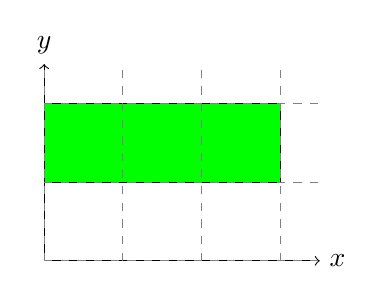
\begin{tikzpicture}
  \draw[black,fill=green] (0,1) rectangle (3,2);
  \draw[->] (0,0)--(3.5,0) node[right]{$x$};
  \draw[->] (0,0)--(0,2.5) node[above]{$y$};
    \begin{scope}
    \clip (0,0) rectangle (3.5,2.5);
    \draw[thin, dashed, gray] (0,0) grid (4,3);
  \end{scope}
\end{tikzpicture}
}

Vypočtěte dvojný integrál $$\iint_\Omega xy^2\mathrm dx\mathrm dy$$
přes obdélník $$
\begin{gathered}
  0\leq x\leq 3\\1\leq y\leq 2.
\end{gathered}
$$

\reseni

$$
\begin{aligned}
  \iint_\Omega xy^2\mathrm dx\mathrm dy
  &=\int_0^3x\,\mathrm dx \int _1^2 y^2 \,\mathrm dy
\\&=\left[\frac {x^2}2\right]_0^3 \times \left[\frac 13 y^3 \right]_1^2
\\&=\left[\frac 92-0\right]\times \left [\frac 13 2^3 - \frac 13 \right]
=\frac 92 \times \frac 73 = \frac {21}2
\end{aligned}
$$


\konec

\subsection{Kvadratický moment pro obdélník}

Vypočtěte integrál
$$
\begin{aligned}
 \iint_\Omega y^2\,\mathrm dx \mathrm dy,\\
\end{aligned}
$$
přes obdélník se stranami podél os, se středem v počátku a délkou stran $a$ a $b$, tj. přes množinu $\Omega$ danou nerovnostmi
$$
\begin{aligned}
  -\frac a2\leq &x\leq \frac a2,\\
  -\frac b2\leq &y \leq \frac b2.
\end{aligned}
$$

\reseni


$$
\begin{aligned}
  \iint_\Omega y^2\,\mathrm dx \mathrm dy
  = \int_{-\frac a2}^{\frac a2} \,\mathrm dx \times \int_{-\frac b2}^{\frac b2}y^2\,\mathrm dy=a\times \left[\frac 13 y^3\right]_{-\frac b2}^{\frac b2}=a\times \left(\frac 13 \times \frac {b^3}{8} + \frac 13 \times \frac {b^3}{8}\right)=
  \frac 1{12}ab^3
\end{aligned}
$$

\konec

\subsection{Integrál závislý na parametru}

\Tobrazek{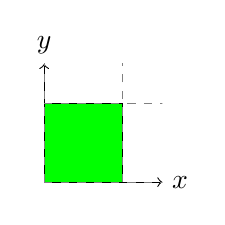
\begin{tikzpicture}
  \draw[black,fill=green] (0,0) rectangle (1,1);
  \draw[->] (0,0)--(1.5,0) node[right]{$x$};
  \draw[->] (0,0)--(0,1.5) node[above]{$y$};
    \begin{scope}
    \clip (0,0) rectangle (1.5,1.5);
    \draw[thin, dashed, gray] (0,0) grid (2,2);
  \end{scope}
\end{tikzpicture}
}

Vypočtěte dvojný integrál $$I_n=\iint_\Omega y^n\mathrm dx\mathrm dy$$
přes jednotkový čtverec $$
\begin{gathered}
  0\leq x\leq 1\\0\leq y\leq 1
\end{gathered}
$$
v závislosti na parametru $n\geq 0$.

\reseni

$$
\begin{aligned}
  \iint_\Omega y^n\mathrm dx\mathrm dy
  &=\int_0^1\,\mathrm dx \int _0^1 y^n \,\mathrm dy
  =1 \times \left[\frac 1{n+1} y^{n+1} \right]_0^1
  =\frac 1{n+1}
\end{aligned}$$


Správnost můžeme ověřit pomocí vzorců pro obsah  $$I_0=1$$ a polohu težiště $$\frac{I_1}{I_0}=\frac 12,$$
což porovnáme s očekávanými výsledky. Dalším využitím je působiště tlakové síly na přehradu (viz přednáška), které je při orientaci osy $y$ od hladiny směrem dolů v místě
$$\frac{I_2}{I_1}=\frac {\frac 13}{\frac 12}=\frac 23,$$
tj. ve dvou třetinách hloubky.

\konec


\subsection{Integrál přes trojúhelník}

\Tobrazek{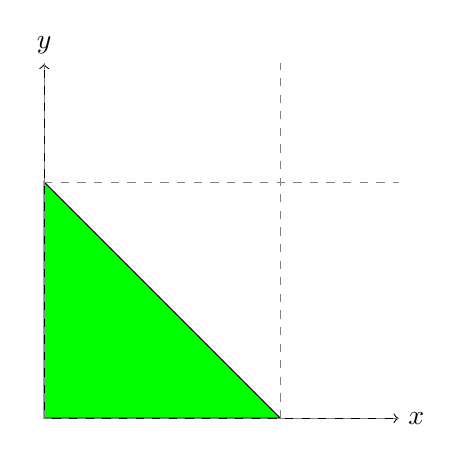
\begin{tikzpicture}[scale=3]
  \draw[black,fill=green, domain=0:1] (0,0) -- (0,1) -- plot ({\x},{1-\x})--cycle;
%  \draw[black,domain=0:1.2] plot ({\x},{1-\x}) node[right]{$y=1-x$};
  \draw[->] (0,0)--(1.5,0) node[right]{$x$};
  \draw[->] (0,0)--(0,1.5) node[above]{$y$};
    \begin{scope}
    \clip (0,0) rectangle (1.5,1.5);
    \draw[thin, dashed, gray] (0,0) grid (4,3);
  \end{scope}
\end{tikzpicture}
}


Vypočtěte integrál
$$  \iint_\Omega xy^2\,\mathrm dx \mathrm dy
$$
přes trojúhelník $\Omega$ s vrcholy v bodech $(0,0)$, $(1,0)$ a $(0,1)$.

\reseni

Rovnice přímky, ve které leží přepona trojúhelníka, je
$$y=1-x$$ a trojúhelník tedy je možno zapsat soustavou nerovností

$$
\begin{aligned}
  0\leq &x\leq 1,\\
  0\leq &y \leq 1-x.
\end{aligned}
$$

Použitím těchto nerovností můžeme dvojný integrál transformovat na dvojnásobný a vypočítat.
$$
\begin{aligned}
  \iint_\Omega xy^2\,\mathrm dx\mathrm dy
  &=\int_0^1 \int_0^{1-x} xy^2\,\mathrm dy\mathrm dx
  =\int_0^1 \left[\frac 13 xy^3\right]_0^{1-x}\,\mathrm dx
  =\int_0^1 \frac 13x(1-x)^3\,\mathrm dx
  \\&=\frac 13 \int_0^1 x-3x^2+3x^3-x^4\,\mathrm dx
  =\frac 13\left[\frac 12 x^2 - x^3 +\frac 34 x^4-\frac 15 x^5\right]_0^1
  \\&=\frac 13\left[\frac 12 -1 +\frac 34 -\frac 15\right] =\frac 1{60}
\end{aligned}
$$

\konec 


\subsection{Integrál pod parabolou}

\Tobrazek{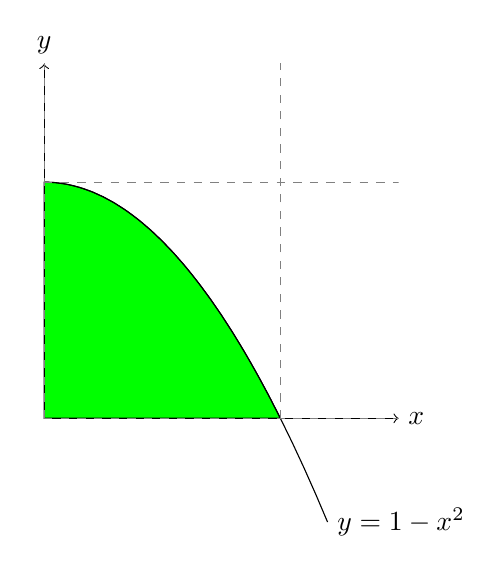
\begin{tikzpicture}[scale=3]
  \draw[black,fill=green, domain=0:1] (0,0) -- (0,1) -- plot ({\x},{1-\x^2})--cycle;
  \draw[black,domain=0:1.2] plot ({\x},{1-\x^2}) node[right]{$y=1-x^2$};
  \draw[->] (0,0)--(1.5,0) node[right]{$x$};
  \draw[->] (0,0)--(0,1.5) node[above]{$y$};
    \begin{scope}
    \clip (0,0) rectangle (1.5,1.5);
    \draw[thin, dashed, gray] (0,0) grid (4,3);
  \end{scope}
\end{tikzpicture}
}


Vypočtěte integrály
$$
\begin{aligned}
  I_1&=\iint_\Omega x\,\mathrm dx \mathrm dy,\\
  I_2&=\iint_\Omega y\,\mathrm dx \mathrm dy,\\
  I_3&=\iint_\Omega \,\mathrm dx \mathrm dy,\\
\end{aligned}
$$
přes množinu $\Omega$ danou nerovnostmi
$$
\begin{aligned}
  0\leq &x\leq 1,\\
  0\leq &y \leq 1-x^2.
\end{aligned}
$$
Určete obsah a polohu těžiště této množiny.

\reseni

$$
\begin{aligned}
  \iint_\Omega x\,\mathrm dx\mathrm dy
  &=\int_0^1 \int_0^{1-x^2} x\,\mathrm dy\mathrm dx
  =\int_0^1 \left[xy\right]_0^{1-x^2}\,\mathrm dx
  =\int_0^1 x(1-x^2)\,\mathrm dx
  =\int_0^1 x-x^3\,\mathrm dx
  \\&=\left[\frac 12 x^2 - \frac 14 x^4\right]_0^1=\frac 12-\frac 14 =\frac 14
\end{aligned}
$$
$$
\begin{aligned}
  \iint_\Omega y\,\mathrm dx\mathrm dy
  &=\int_0^1 \int_0^{1-x^2} y\,\mathrm dy\mathrm dx
  =\int_0^1 \left[\frac 12 y^2\right]_0^{1-x^2}\,\mathrm dx
  =\int_0^1 \frac 12 (1-x^2)^2\,\mathrm dx
  \\&=\frac 12 \int_0^1 1-2x^2+x^4\,\mathrm dx
  =\frac 12 \left[x-\frac 23 x^3 + \frac 15 x^5\right]_0^1=\frac 12\left[1-\frac 23 + \frac 15\right]=\frac 4{15}
\end{aligned}
$$

$$
\begin{aligned}
  \iint_\Omega \,\mathrm dx\mathrm dy
  &=\int_0^1 \int_0^{1-x^2} \,\mathrm dy\mathrm dx
%  =\int_0^1 \left[y\right]_0^{1-x^2}\,\mathrm dx
  =\int_0^1 1-x^2\,\mathrm dx
  =\left[x - \frac 13 x^3\right]_0^1=1-\frac 13 =\frac 23
\end{aligned}
$$

Obsah je $\frac 23$ a souřadnice těžiště jsou $\left[\frac 38,\frac 4{10}\right]$. Toto je možné porovnat s obsahem a souřadnicemi těžiště trojúhelníka, který vznikne nahrazením paraboly přímkou a tento trojúhelník má obsah $\frac 12$ a souřadnice těžiště $\left[\frac 13,\frac 13\right].$

\konec 
\subsection{Integrál přes čtvrtkružnici}

\let\phi \varphi
\Tobrazek{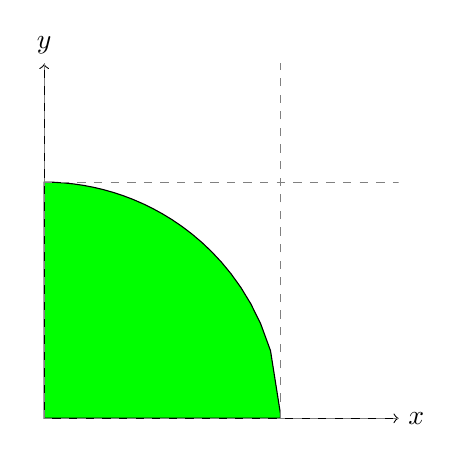
\begin{tikzpicture}[scale=3]
  \draw[black,fill=green, domain=0:1] (0,0) -- (0,1) -- plot ({\x},{sqrt(1-\x^2)})--(1,0)--cycle;
  \draw[->] (0,0)--(1.5,0) node[right]{$x$};
  \draw[->] (0,0)--(0,1.5) node[above]{$y$};
    \begin{scope}
    \clip (0,0) rectangle (1.5,1.5);
    \draw[thin, dashed, gray] (0,0) grid (4,3);
  \end{scope}
\end{tikzpicture}
}


Vypočtěte integrály
$$
\begin{aligned}
  I_1&=\iint_\Omega x\,\mathrm dx \mathrm dy,\\
  I_2&=\iint_\Omega y\,\mathrm dx \mathrm dy,\\
  I_3&=\iint_\Omega \,\mathrm dx \mathrm dy,\\
\end{aligned}
$$
přes čtvrtkružnici na obrázku (čtvrtina jednotkové kružnice v prvním kvadrantu).
Určete obsah a polohu těžiště této čtvrtkružnice.

\reseni

V polárních souřadnicích daných rovnicemi $$
\begin{aligned}
  x&=r\cos\phi\\
  y&=r\sin\phi
\end{aligned}
$$
má čtvrtkružnice vyjádření $0\leq r\leq 1$, $0\leq \phi\leq \frac \pi2$.
$$
\begin{aligned}
  \iint_\Omega x\,\mathrm dx\mathrm dy
  &=\int_0^1 \int_0^{\frac \pi2} r\cos\phi \times r\,\mathrm d\phi\mathrm dr
  =\int_0^1 r^2 \,\mathrm dr \times \int_0^{\frac \pi2}\cos\phi \mathrm d \phi
  \\&=\left[\frac 13 r^3\right]_0^1\times \left[\sin\phi\right]_0^{\frac \pi2}=\frac 13 \times 1=\frac 13
\end{aligned}
$$$$
\begin{aligned}
  \iint_\Omega y\,\mathrm dx\mathrm dy
  &=\int_0^1 \int_0^{\frac \pi2} r\sin\phi \times r\,\mathrm d\phi\mathrm dr
  =\int_0^1 r^2 \,\mathrm dr \times \int_0^{\frac \pi2}\sin\phi \mathrm d \phi
  \\&=\left[\frac 13 r^3\right]_0^1\times \left[-\cos\phi\right]_0^{\frac \pi2}=\frac 13 \times 1=\frac 13
\end{aligned}
$$
$$
\begin{aligned}
  \iint_\Omega \,\mathrm dx\mathrm dy
  &=\int_0^1 \int_0^{\frac \pi2} 1 \times r\,\mathrm d\phi\mathrm dr
  =\int_0^1 r \,\mathrm dr \times \int_0^{\frac \pi2}\mathrm d \phi
  \\&=\left[\frac 12 r^2\right]_0^1\times {\pi2}=\frac 12 \times \frac \pi 2=\frac \pi 4
\end{aligned}
$$

Obsah je $\frac \pi 4$, což odpovídá čtvtině vzorce pro obsah jednotkového kruhu. Souřadnice težište jsou obě stejné, což odpovídá symetrii množiny.  Tyto souřadnice leží v bodě
$$\frac {4}{3\pi}\approx 0.42,$$
což odpovídá tomu, že těžište je posunuto doprava nahoru ve srovnání těžištěm trojúhelníka, který by vznikl nahrazením oblouku úsečkou.

\konec

\subsection{Kvadratický moment kruhu}

Vypočtěte kvadratický moment kruhu o poloěmru $R$ vzhledem k ose procházející středem.

\reseni

Vypočteme kvadratický moment kruhu daného v polárních souřadnicích nerovnicemi
$$
\begin{aligned}
  0&\leq r\leq R,\\
  0&\leq \varphi\leq 2\pi.  
\end{aligned}
$$

Přímým výpočtem dostáváme
$$
\begin{aligned}
  \iint_{\Omega}y^2\,\mathrm dx\mathrm dy&=
  \int_{0}^R \int_0^{2\pi} r^2\sin^2\varphi \times r\,\mathrm d\varphi \mathrm dr
  =\int_{0}^R  r^3  \mathrm dr \int_0^{2\pi}\sin^2\varphi \,\mathrm d\varphi
  =\left[\frac {r^4}{4}\right]_0^R \pi
  =\frac {\pi}{4} R^4,
\end{aligned}
$$
kde při výpočtu integrálu přes proměnnou $\varphi$ využijeme nápovědu, kterou jsme měli již v sadě úloh s křivkovým integrálem.

Že je výsledkem veličina úměrná čtvrté mocnině poloměru je zřejmé i z rozměrové analýzy (resp. z Buckinghamova $\Pi$ teorému), uvedeným výpočtem však vidíme i konstantu úměrnosti.

To že kvadratický moment roste se čtvrtou mocninou poloměru značí, že snížení průměru tyče na polovinu vede k redukci tuhosti na přibližně $(0.5)^4$ tj. na šest procent. Devadesát šest procent tuhosti je v materiálu, který se při tomto odstraní. Proto jsou trubky při stejné spotřebě materiálu odolnější vůči ohnutí než tyče. Proto mají listy rostlin nebo listy vrtulí větrných elektráren materiál odpovídající za tuhost na povrchu. Proto máme kosti duté.

\konec


%

%\subsection{Jacobiho matice pro polární souřadnice}

%  Najděte Jacobiho matici a její determinant pro transformaci 
% \begin{equation*}
%   \begin{aligned}
%     x&=r\cos \varphi\\
%     y&=r\sin \varphi
%   \end{aligned}
% \end{equation*}
% mezi polárními a kartézskými souřadnicemi.



\section{Křivkový integrál pomocí potenciálu, Greenova věta, rovnice kontinuity}


\subsection{Křivkový integrál pomocí kmenové funkce}


Určete, pro jako hodnotu parametru $a\in \mathbb R$ křivkový integrál vektorového pole $$\vec F=ax^2y\vec\imath + (x^3+1)\vec\jmath$$ po křivce $C$, tj. $$\int_C ax^2y\,\mathrm dx+(x^3+1)\,\mathrm dy$$ nezávisí na integrační cestě v $\mathbb R^2$. Najděte kmenovou funkci příslušného vektorového pole a vypočtěte křivkový integrál po křivce z bodu $[0,0]$ do bodu $[1,2]$.

\reseni

Podmínka pro nezávislost na integrační cestě je $$
\begin{aligned}
0&=\nabla \times  \vec F
=\begin{vmatrix}
  \vec i & \vec j& \vec k \\
  \frac{\partial}{\partial x} &  \frac{\partial}{\partial y} &  \frac{\partial}{\partial z}\\
  ax^2y &  x^3+1 &  0
\end{vmatrix}
\\&=\vec k \left(  \frac{\partial}{\partial x} (x^3+1) - \frac{\partial }{\partial y} (ax^2y)\right)
  =\vec k(3x^2-ax^2y)=\vec k x^2(3-a)
\end{aligned}
  $$
  a odsud $a=3$. Totéž dokážeme určit pomocí věty, kterou jsme se ukázali již v souvislosti s pojmem gradient, ze které vyplývá podmínka na existenci kmenové funkce ve tvaru $$
\begin{aligned}
  \pdv{y}(ax^2y)&=\pdv{x}(x^3+1)\\
  ax^2&=3x^2\\
  a&=3
\end{aligned}
$$
Kmenová fukce $\varphi(x,y)$ vektorového pole $\vec F=(3x^2y,x^3+1)$ splňuje
$$
\begin{aligned}
  \pdv{\varphi}{x}&=3x^2y \\  \pdv{\varphi}{y}&=x^3+1.
\end{aligned}
$$
Integrací dostáváme
$$
\begin{aligned}
  \varphi &= \int 3x^2y\,\mathrm dx=x^3y+C_1(y)\\
  \varphi &= \int x^3+1\,\mathrm dy=x^3y+y+C_2(x)
\end{aligned}
$$
Porovnáním dostáváme kenovou funkci $$\varphi (x,y)=x^3y+y+C,$$ kde $C$ je integrační konstanta. Integrál po křivce (tvar není důležitý, vzhledem k nezávislosti na integrační cestě stačí počáteční a koncový bod) je
$$\int _C \vec F\mathrm d\vec r=\varphi(1,2)-\varphi(0,0)=2+2-0=4.$$


\konec

\subsection{Křivkový integrál pomocí kmenové funkce 2}

Pro jakou hodnotu parametru $m$ je křivkový integrál
$$\int (6x^2y+x+y)\,\mathrm dx+(mx^3+x)\,\mathrm dy$$ nezávislý na
integrační cestě v $\mathbb R^2$? Vypočtěte hodnotu tohoto integrálu
po křivce z bodu $(2,1)$ do bodu $(1,3)$.

\reseni

Podmínka pro nezávislost na integrační cestě je $$\pdv{y}\qty(6x^2y+x+y)=\pdv{x}\qty(mx^3+x).$$
Po výpočtu derivací dostáváme
$$6x^2+1=3mx^2+1$$
a odsud $m=2$.

Hledáme funkci, jejímž gradientem je vektorové pole $\vec F=(6x^2y+x+y,2x^3+x)$. 
Integrací podle $x$ a podle $y$ dostáváme
$$\int (6x^2y+x+y)\,\mathrm dx= 2x^3y+\frac 12 x^2+xy+C_1(y) $$
a
$$\int (2x^3+x)\,\mathrm dy=2x^3y+xy+C_2(x).$$
Porovnáním získáme kmenovou funkci
$$\varphi(x,y)=2x^3y+\frac 12 x^2+xy+C,
\quad C
\in
\mathbb R.$$

Integrál po křivce  z bodu $(2,1)$ do bodu $(1,3)$
má hodnotu
$$\varphi(1,3)-\varphi(2,1)=6+\frac 12 +3-\qty(16+2+2)=-\frac{21}2.$$

\konec


\subsection{Kmenová funkce pomocí křivkového integrálu}

Ukažte, že vektorové pole
$\vec F=(6x^2y+x+y,2x^3+x)$ má kmenovou funkci. Vypočtěte z definice křivkový integrál v tomto vektorovém poli po křivce $\vec r(t)=(at,bt)$, $t\in[0,1]$, tj. po úsečce z počátku do bodu $(a,b)$ a ukažte, že tímto způsobem obdržíme kmenovou funkci.  

\reseni
Platí $$\pdv{y}\qty(6x^2y+x+y)=6x^2+1=\pdv{x}\qty(2x^3+x)$$
a proto kmenová funkce existuje.

Derivací křivky dostáváme rovnici tečného vektoru
$$\frac{\mathrm d\vec r}{\mathrm dt}=(a,b)$$
a dosazením křivky do vektorového pole
$$\vec F(\vec r(t))=(6a^2t^2bt+at+bt,2a^3t^3+at)=(6a^2bt^3+at+bt,2a^3t^3+at).$$
Skalární součin je daný vztahem
$$\vec F\frac{\mathrm d\vec r}{\mathrm dt}=a(6a^2bt^3+at+bt)+b(2a^3t^3+at)
=8a^3b t^3+a^2t+2abt.
$$
Křivkový integrál je tedy roven
$$\int_C \vec F\,\mathrm d\vec r=
\int_0^1 8a^3b t^3+a^2t+2abt\,\mathrm dt=
\qty[2a^3bt^4+\frac 12 a^2 t^2+abt^2]_0^1=2a^3b+\frac 12 a^2+ab.
$$
Podle věty o nezávislosti křivkového integrálu na integrační cestě máme
$$\varphi(a,b)-\varphi(0,0)=2a^3b+\frac 12 a^2+ab$$
a odsud
$$\varphi(a,b)=2a^3b+\frac 12 a^2+ab+\varphi(0,0),$$
neboli (po přejmenování proměnných a zavedení konstanty $C$ místo $\varphi(0,0)$)
$$\varphi(x,y)=2x^3y+\frac 12 x^2+xy+C.$$

\konec

\subsection{Greenova věta}

Určete integrál $$\oint_C \vec F\,\mathrm d\vec r$$ po křivce, která je kladně orientovanou hranicí jednotkového čtverce s vrcholy v bodech $(0,0)$, $(1,0)$, $(0,1)$, $(1,1)$ pro vektorovou funkci $$\vec F=x^7\vec i+xy\vec j.$$

\reseni

$$
\begin{aligned}
  \oint_C \vec F\,\mathrm d\vec r
  &=
  \oint_C x^7\,\mathrm dx+ xy\,\mathrm dy\\&
  =\int_0^1 \int_0^1 \frac{\partial}{\partial x}(xy)-\frac{\partial}{\partial y}(x^7) \,\mathrm dy\mathrm dx\\
  &=\int_0^1 \int_0^1 y \,\mathrm dy\mathrm dx\\&
  =\int_0^1 y \,\mathrm dy \times \int_0^1 \,\mathrm dx \\&= \left[\frac 12 y^2\right]_0^1 \times 1\\&= \frac 12
\end{aligned}
$$

\konec

\subsection{Rovnice vedení tepla v materiálech různých vlastností}

Rovnice vedení tepla v ortotropním materiálu umístěném do souřadné soustavy tak, aby vlastní směry tenzoru tepelné vodivosti (jako např. anatomické směry dřeva) má nejobecnější možné vyjádření
$$c\rho\pdv{T}{t}=\pdv{x}\qty(\lambda_x\pdv{T}{x} )+\pdv{y}\qty(\lambda_y\pdv{T}{y}) . $$
Za jakých okolností je možno veličiny $\lambda_x$ a $\lambda_y$ napsat před vnější derivaci tak, aby v rovnici vznikly druhé derivace? 


\obrazek{chladic.jpg}
\subsection{Stacionární vedení tepla v žebru chladiče}

Vyjímečně jsme nuceni do rovnice vedení tepla zahrnout i zdroje. 
Modelujte vedení tepla v žebru chladiče. Úlohu uvažujte jako
jednorozměrnou, materiál homogenní izotropní s konstantní tepelnou
vodivostí. Kolem chladiče proudí vzduch a teplotě $T_0$ a chladič
ztrácí teplo rychlostí úměrnou rozdílu teploty žebra v daném místě a
teploty okolního vzduchu. (Koeficient úměrnosti je dán koeficient přestupu tepla a šířkou žebra).


\section{Diferenciální rovnice I}

\obrazek{mladata.jpg}
\subsection{Model růstu úměrného velikosti chybějícího množství}  \label{krava}
Mnoho
živočichů roste tak, že mohou dorůstat jisté maximální délky a
rychlost jejich růstu je úměrná délce, která jim do této maximální
délky chybí (tj. kolik ještě musí do této maximální délky
dorůst). Sestavte matematický model popisující takovýto růst.


\textit{Jakmile vidíme, že v zadání figuruje rychlost změny veličiny,
  která nás zajímá, je jasné, že kvantitativní model bude obsahovat
  derivaci. Zatím se učíme model zapsat, později ho budeme umět i vyřešit.}


\reseni
Je-li $L$ délka a $L_{\max}$ maximální délka, potom do maximální délky chybí  $L_{\max}-L$ a model má tvar
$$\derivace Lt=k (L_{\max}-L).$$
\konec

\obrazek{kontaminace.jpg}
\subsection{Kontaminace a čištění}
%Hughes
Znečišťující látky se v kontaminované oblasti rozkládají tak, že za den se samovolně rozloží 
$8\%$ aktuálního znečištění. Kromě toho pracovníci odstraňují látky rychlostí $30$
galonů denně. Vyjádřete tento proces kvantitativně pomocí vhodného
modelu.

\textit{Tento příklad opět zmiňuje rychlost změny, tj. derivaci. Tentokrát se na změně podílejí dva procesy a jejich účinek se sčítá. Příklad navíc připomíná, jak se pracuje se změnou vyjádřenou procenty. Toto je používané například při úročení spojitým úrokem. Pokud pokles změníme na růst, tj. pokud změníme
  znaménka u derivace, máme okamžitě model růstu financí na účtu, na kterém se pravidelně připisuje úrok a k tomu se přidává fixní úložka.}

\reseni Je-li $y$ znečištění v galonech a $t$ čas ve dnech, má model tvar
$$\derivace yt=-0.08y-30.$$

\konec



\obrazek{lov.jpg}
\subsection{Logistická rovnice: model využívání přírodních zdrojů}
Při modelování růstu populace o velikosti $x(t)$ často pracujeme s populací žijící v prostředí s omezenou úživností (nosnou kapacitou). Často používáme model
$$\frac{\mathrm d x}{\mathrm dt}=rx\left(1-\frac xK\right),$$
kde $r$ a $K$ jsou parametry modelu (reálné konstanty).  Nakreslete
graf funkce $f(x)=rx\left(1-\frac xK\right)$ a ověřte, že pro velká
$x$ je $f(x)$ záporné a velikost populace proto klesá. Pokud populaci
lovíme konstantní rychlostí, sníží se pravá strana o konstantu, kterou
označíme $h$. Ukažte, že pro intenzivní lov bude pravá strana rovnice
pořád záporná a intenzivní lov tak způsobí vyhubení populace. Dá se
najít kritická hodnota lovu oddělující vyhynutí populace a její
trvalé přežívání?

\textit{Toto je asi nejdůležitější rovnice pro modelování biologických jevů. Používá se při modelování vývoje obnovitelných zdrojů a bývá modifikována pro konkrétní případy podle toho, jak populace interaguje s okolím.}

\reseni
Funkce $f(x)=rx\left(1-\frac xK\right)$ je kvadratická funkce s nulovými body $x=0$ a $x=K$, vrcholem uprostřed mezi nulovými body (tj. pro $x=\frac K2$) a parabola je otočená vrcholem nahoru. Proto je napravo od $x=K$ záporná. To odpovídá tomu, že populace s velikostí přesahující nosnou kapacitu v dlouhodobém horizontu vymírá.

Funkce $f_h(x)=rx\left(1-\frac xK\right)-h$ vznikne posunutím funkce $f(x)=rx\left(1-\frac xK\right)$ o $h$ dolů. Pokud posuneme hodně, dostane se celá parabola pod osu $x$ a funkce bude pořád záporná. Kritická hodnota je v situaci, kdy mizí možnost, že $f_h(x)$ má body kde je kladná a populace se může rozvíjet. To nastane,  pokud se vrchol paraboly dostane na osu $x$, tj. $h$ je rovno funkční hodnotě funkce $f(x)$ v bodě $x=\frac K2.$
\konec



\stranka

\obrazek[pixabay.com, autor Free-Photos]{deer.jpg}

\subsection{Populace jelenů}

 Populace jelenů v~národním parku přibývá rychlostí 10\% za
    rok. Správa parku každý rok odebere 50 jedinců. Napište
    matematický model pro velikost populace jelenů v~tomto parku.

    \reseni
    Je-li $x$ velikost populace jelenů, platí
    \begin{equation*}
      \derivace xt=0.10 x-50, 
    \end{equation*}
    kde $t$ je čas v letech.
\konec


%\obrazek{nemoc.jpg}
\subsection{Hrubý model chřipkové epidemie}  Rychlost
s jakou roste počet nemocných chřipkou je úměrný současně počtu
nemocných a počtu zdravých jedinců. Sestavte model takového šíření
chřipky.

\textit{Toto je současně model popisující šíření informace v populaci, stačí si místo chřipky představit nějakou informaci předávanou mezi lidmi (sociální difuze).}

\reseni
Je-li $M$ velikost populace a $y$ počet nemocných, je v populaci $M-y$ zdravých a model má tvar
$$\derivace yt=ky(M-y).$$

\konec



\obrazek{olej.jpg}

\subsection{Ropná skvrna} Kruhová ropná skvrna na hladině se rozšiřuje
tak, že její poloměr jako funkce času roste rychlostí, která je
nepřímo úměrná druhé mocnině poloměru. Vyjádřete proces kvantitativně
pomocí derivací.

\reseni
Je-li $r$ poloměr, je $r^2$ druhá mocnina a protože se jedná o nepřímou úměrnost, platí
$$\derivace rt=\frac{k}{r^2}.$$
\konec

\subsection{Model učení} Rychlost učení (tj. časová změna objemu
osvojené látky nebo procento z~maximální manuální zručnosti) je úměrná
objemu dosud nenaučené látky. Vyjádřete proces kvantitativně pomocí
derivací.

\textit{Porovnejte s příkladem \ref{krava}.}

\reseni
Je-li $L$ objem naučené látky a $L_{\max}$ maximální objem látky kterou je možné se naučit, je objem dosud nenaučené látky $L_{\max}-L$ a model má tvar
$$\derivace Lt=k (L_{\max}-L).$$
\konec

\stranka

\subsection{Řešení ODE a IVP} 

\begin{multicols}2

\def\priklad #1. {$#1$}

\begin{enumerate}[(1)]
  \setlength\itemsep{10pt}
\item \priklad \frac{\mathrm dy}{\mathrm dx}=xy^2.
\item \priklad \frac{\mathrm dy}{\mathrm dt}=te^y.
\item \priklad \frac{\mathrm dy}{\mathrm dx}=x\sqrt y.
\item \priklad \frac{\mathrm dy}{\mathrm dx}=x\sqrt y,\ \ y(0)=1.
\item \priklad \frac{\mathrm dr}{\mathrm dt}=kr^3,\ \ r(0)=r_0>0.
\item \priklad \frac{\mathrm dm}{\mathrm dt}=m+2,\ \ m(0)=0.
\item \priklad \frac{\mathrm dm}{\mathrm dt}=m+2,\ \ m(0)=-2.
\end{enumerate}
\end{multicols}

\textit{Umění najít řešení diferenciální rovnice je sympatické, není to však nic proti umění sestavit model (naučili jsme se již ve druhém týdnu, připomeneme si v následujícím modelu), umění posoudit jednoznačnost řešení (většina modelů se řeší numericky a musíme být přesvědčeni o smysluplnosti takové činnosti) a  stabilitu řešení (řešení, která nejsou stabilní, jsou sice v souladu s přírodními zákony, ale pravděpodobnost jejich spontánního výskytu je nulová). Jednoznačnost a zjednodušenou verzi stability řešení (stabilita konstantních řešení) jsme viděli na přednášce a připomeneme v dalších příkladech.}

\stranka

\def\priklad #1.{$#1$}

\reseni

\begin{enumerate}[(1)]
\item \priklad \frac{\mathrm dy}{\mathrm dx}=x\cdot y^2.
  \begin{itemize}
  \item Konstantní řešení jsou řešení rovnice $$ y^2=0,$$ tj. je jediné konstantní řešení $$ y=0.$$
  \item Pro nekonstantní řešení dostaneme po separaci  $$ y^{-2}\mathrm dy=x\mathrm dx $$ a integrováním $$ -\frac 1y=\frac 12 x^2+C.$$
  \end{itemize}
\item \priklad \frac{\mathrm dy}{\mathrm dt}=t\cdot e^y.
  \begin{itemize}
  \item Konstantní řešení jsou řešení rovnice $$ e^y=0.$$ Protože tato rovnice nemá řešení, zadaná diferenciální rovnice nemá konstantní řešení.
  \item Pro nekonstantní řešení dostaneme po separaci  $$ e^{-y}\mathrm dy= t\mathrm dt$$ a integrováním $$ -e^{-y}=\frac 12 t^2 +C.$$
  \end{itemize}
\item \priklad \frac{\mathrm dy}{\mathrm dx}=x\cdot \sqrt y.
  \begin{itemize}
  \item Konstantní řešení jsou řešení rovnice $$ \sqrt y=0,$$ tj. jediné řešení $$ y=0.$$
  \item Pro nekonstantní řešení dostaneme po separaci  $$ \frac 1{\sqrt y}\mathrm dy=x\mathrm dx $$ a integrováním $$ 2\sqrt y=\frac 12 x^2+C.$$
  \end{itemize}
\item \priklad \frac{\mathrm dy}{\mathrm dx}=x\sqrt y,\ \ y(0)=1.
  \begin{itemize}
  \item Konstantní řešení $$y=0$$ (viz předcdhozí příklad) nesplňuje počáteční podmínku a proto jej nemusíme uvažovat
  \item Obecné řešení  $$ 2\sqrt y=\frac 12x^2 +C$$ dává po dosazení $x=0$ a $y=1$ rovnici $$2\sqrt 1=0+C.$$ Odsud dostáváme $C=2$ a řešení zadané počáteční úlohy je $$2\sqrt y=\frac 12 x^2+2.$$
  \end{itemize}
\item \priklad \frac{\mathrm dr}{\mathrm dt}=k\cdot r^3,\ \ r(0)=r_0>0.
  \begin{itemize}
  \item Konstantní řešení jsou řešení rovnice $$ r^3=0,$$ tj. jediné konstantní řešení je $$ r=0$$ a toto řešení nesplňuje počáteční podmínku.
  \item Pro nekonstantní řešení dostaneme po separaci  $$ r^{-3}\mathrm dr=k\mathrm dt $$ a integrováním $$ -\frac 12 r^{-2}=kt+C.$$ Dosazením počáteční podmínky $t=0$, $r=r_0$ dostáváme $$ -\frac 12 r_0^{-2}=C.$$ Tím je dána konstanta $C$ a po použití této konstanty v obecném řešení dostáváme řešení počáteční úlohy ve tvaru $$ -\frac 12 r^{-2}=kt-\frac 12 r_0^{-2}.$$
  \end{itemize}
\item \priklad \frac{\mathrm dm}{\mathrm dt}=m+2,\ \ m(0)=0.
  \begin{itemize}
  \item Konstantní řešení jsou řešení rovnice $$ m+2=0$$, tj. $$ m=-2$$ a toto řešeín nesplňuje počáteční podmínku.
  \item Pro nekonstantní řešení dostaneme po separaci  $$ \frac1{m+2}\mathrm dm=dt $$ a integrováním $$ \ln|m+2|=t+C.$$ Po dosazení počáteční podmínky $t=m=0$ dostáváme $$C=\ln 2$$ a počáteční úloha má řešení $$\ln(m+2)=t+\ln (2).$$ (Vzhledem k počáteční podmínce je $y$ kladné a nemusíme psát integrační konstantu.)
  \end{itemize}
\item \priklad \frac{\mathrm dm}{\mathrm dt}=m+2,\ \ m(0)=-2.
  \begin{itemize}
  \item Konstantní řešení jsou řešení rovnice $$ m+2=0$$, tj. $$ m=-2.$$ Toto 5e3ení splňuje počáteční podmínku.
  \item Pravá strana má ohraničenou (dokonce konstantní) derivaci podle $m$. Proto je řešení každé počáteční úlohy určeno jednozančně. Řešení z předchozího bodu je jediné a další nemusíme hledat.
  \end{itemize}
\end{enumerate}

\konec

\obrazek{ledni_medved.jpg}
\subsection{Tloušťka ledu}

Takzvaný Stefanův zákon (J. Stefan, \"Uber die Theorie der Eisbildung, insbesondere \"uber die Eisbildung im Polarmeere, 1891) vyjadřuje že tloušťka ledu na hladině moře roste ve
stabilních podmínkách rychlostí nepřímo úměrnou této tloušťce. Zapište
tento fakt pomocí vhodného matematického modelu a najděte řešení
vzniklé diferenciální rovnice.

\reseni

$$
\begin{aligned}
\frac{\mathrm dh}{\mathrm dt}&=\frac kh\\
h\,\mathrm dh&=k\, \mathrm dt\\
\int h\,\mathrm dh&=\int k\, \mathrm dt\\
\frac {h^2}{2}&=kt+C\\
\end{aligned}
$$



\konec 


\stranka

\obrazek[www.rodovystatek.cz]{voda_plastovky.jpg}[-10pt]
\subsection{Model vypouštění nádrže} \label{vypousteni} Z fyziky je známo, že rychlost s jakou
vytéká tekutina otvorem u dna nádoby je úměrná odmocnině výšky hladiny
(protože se mění potenciální energie úměrná výšce na kinetickou
energii úměrnou druhé mocnině rychlosti). Proto je i rychlost s jakou
se zmenšuje objem vody v nádrži úměrná odmocnině výšky
hladiny.

Ukažte, že matematickým popisem procesu je diferenciální rovnice.
Napište rovnici pro výšku hladiny vody v nádrži jako funkci času.
Uvažujte tři případy:
nádrž \textbf{cylindrického tvaru} (válec postavený na podstavu),
nádrž ve tvaru
\textbf{kvádru} 
a nádrž ve tvaru \textbf{kužele} otočeného vrcholem dolů (trychtýř). 


\textit{V tomto příkladě vystupuje derivace jak rychlost, ale po přepisu zadání do modelu máme v rovnici dvě různé veličiny, které se mění: objem vody a výšku hladiny. Musíme ještě najít a použít vztah mezi rychlostmi změn těchto veličin. Fyzikální zákon je formulován pro derivaci objemu a nás zajímá derivace výšky.}

\reseni
Buď $V$ objem vody a $h$ výška hladiny od dna.
Podle zadání ve všech případech platí $$\frac {\mathrm dV}{\mathrm dt}=-k_1\sqrt h$$ a musíme derivaci $\frac {\mathrm dV}{\mathrm dt}$ vyjádřit pomocí $\frac {\mathrm dh}{\mathrm dt}$.

Pro cylindr, kvádr nebo jakoukoliv nádrž se svislými stěnami je objem úměrný výšce hladiny, $V=k_2 h$, a proto $\frac {\mathrm dV}{\mathrm dt}=k_2\frac {\mathrm dh}{\mathrm dt}$. Odsud
$$k_2\frac {\mathrm dh}{\mathrm dt}=\frac {\mathrm dV}{\mathrm dt}=-k_1\sqrt h,$$
tj.
$$\frac {\mathrm dh}{\mathrm dt}=-\frac{k_1}{k_2}\sqrt h$$
a pro $k=\frac{k_1}{k_2}$ má model tvar
$$\frac {\mathrm dh}{\mathrm dt}=-k\sqrt h.$$

Pro kužel platí $V=k_3h^3$ (díky podobnosti je objem přímo úměrný třetí mocnině libovolného délkového parametru) a proto
$\frac {\mathrm dV}{\mathrm dt}=k_3 \times 3h^2 \frac {\mathrm dh}{\mathrm dt}$.
Odsud
$$3k_3 h^2 \frac {\mathrm dh}{\mathrm dt}=\frac {\mathrm dV}{\mathrm dt}=-k_1\sqrt h,$$
tj. 
$$\frac {\mathrm dh}{\mathrm dt}=-\frac{k_1}{3k_3}h^{-3/2}$$
a po přeznačení konstanty má model pro kuželovou nádrž tvar
$$\frac {\mathrm dh}{\mathrm dt}=-kh^{-3/2}.$$


\konec

\stranka
\obrazek[www.rodovystatek.cz]{voda_plastovky.jpg}[-30pt]


\subsection{Problematika jednoznačnosti v modelu vypouštění nádrže}

Ve cvičení \ref{vypousteni}  jsme odvodili rovnici
$$\derivace ht=-k\sqrt h$$
popisující úbytek hladiny vody v nádrži tvaru kvádru, ze které vypouštíme vodu.
\begin{enumerate}[A)]
\item Zkontrolujte, že pro $h>0$ má každá počáteční úloha jediné řešení. Interpretujte tento výsledek prakticky.
\item Pro $h=0$ by řešení nemuselo být určeno jednoznačně. A opravdu
  není. Řešením je například $h(t)=0$ nebo $$h(t)=
  \begin{cases}
    \frac 14 k^2 t^2 & t<0\\
    0 & t\geq 0.
  \end{cases}
  $$
Zkontrolujte dosazením (pozor: pro $t<0$ platí $\sqrt {t^2}=|t|=-t$) a rozmyslete, jestli nejednoznačnost je jenom matematický trik, nebo jestli má
 fyzikální interpretaci.
\end{enumerate}

\reseni
\begin{enumerate}[A)]
\item Nabídneme dvě  varianty, pro argumentaci je možno použít kteroukoliv z nich. 
  \begin{itemize}
  \item \textbf{Podle obecné věty o jednoznačnosti:} Stačí ověřit, že pravá strana má ohraničenou parciální derivaci podle $h$. Protože platí
    $$\frac{\partial }{\partial h}(k\sqrt h)=k\frac 12
    h^{-1/2}=\frac{k}{2\sqrt h}$$ a tato derivace je definovaná a
    ohraničená v nějakém okolí libovolného bodu splňujícího $h>0$.
    Podle věty o existenci a jednoznačnosti řešení obecné
    diferenciální rovnice má počáteční úloha právě jedno řešení.
  \item \textbf{Podle věty o jednoznačnosti pro rovnici se separovanými proměnnými: } Stačí ověřit,
    že část závislá na $h$ je nenulová. Toto jistě platí, protože pro
    $h>0$ je $\sqrt{h}\neq 0$.
\end{itemize}
Pokud je tedy v nádrži nějaká voda, je jednoznačně dáno,
    jak bude vytékat a je možné vypočítat, jaká bude v libovolném
    okamžiku hladina.
  
\item
  Pro $h=\frac 14 k^2 t^2$ a $t<0$ dostáváme
  \begin{equation*}
    \begin{aligned}
      \derivace ht&=\frac 14 k^2 \cdot 2t = \frac 12 k^2 t\\
      -k\sqrt h&=-k\sqrt{\frac 14 k^2 t^2} = - k \frac 12 |k| \cdot |t| =
      - k \frac 12 k (-t) = \frac 12 k^2 t
    \end{aligned}
  \end{equation*}
  a obě strany rovnice jsou stejné. Pro $h=0$ je dosazení triviální.
  
  Je-li $h(t_0)=0$, může to být proto, že voda v čase $t_0$ právě vytekla, nebo proto, že vytekla před hodinou nebo proto, že v nádrži nikdy voda nebyla. Proto je nejednoznačnost přirozená. Například $h(t)=0$ je řešení odpovídající tomu, že voda v nádrži nikdy nebyla. Funkce $h(t)=\frac 14 k^2t^2$ pro $t<0$ odpovídá tomu, že pro $t<0$ v nádrži voda byla a vytekla v čase $t=0$.
\end{enumerate}

\konec


\stranka

\obrazek[vlastní]{pokros.jpg}


\subsection{Stavebniny vedle čebínského nádraží: model} Hromada sypkého
materiálu má tvar kužele. Úhel u~vrcholu je konstantní, daný
mechanickými vlastnostmi materiálu a je nezávislý na
objemu. Předpokládejme, že personál stavebnin přisypává na hromadu
materiál konstantní rychlostí (v jednotkách objemu za jednotku
času). Tato hromada je však v poměrně otevřené krajině a vítr
rozfoukává materiál po okolí. Je rozumné předpokládat, že rozfoukávání (opět v jednotkách objemu za jednotku
času)
se děje rychlostí úměrnou povrchu návětrné strany pláště. Vyjádřete proces kvantitativně pomocí derivací.
Napište rovnici pro derivaci objemu hromady podle času. 

\textit{Toto je podobný model jako model vypouštění nádrže, ale kratší. Opět máme po přepisu zadání do matematického modelu dvě veličiny měnící se s časem v jedné rovnici. Derivace objemu, která nás zajímá, již v rovnici přítomna naštěstí je. Stačí vyjádřit obsah pomocí objemu, nejlépe pomocí rozměrové analýzy.}

\reseni
Rychlost s jakou se mění objem je $\frac{\mathrm dV}{\mathrm dt}$, rychlost přisypávání označme $R$, povrch návětrné strany $S$.
Podle zadání platí
$$  \frac{\mathrm dV}{\mathrm dt} = R - k_0S.$$
Protože kužel má stále stejný tvar, objem jednoznačně determinuje rozměry, povrch kužele, nebo i povrch poloviny pláště, tj. povrch návětrné strany. Z rozměrové analýzy na základě Buckinghamova Pi-teorému z přednášky je zřejmé, že musí platit úměrnost mezi takovými mocninami těchto veličin, pro které jednotky ``pasují'', Existuje tedy konstanta taková, že $$S=k_1V^{\frac 23}.$$ Spojením těchto dvou vztahů dostáváme
$$  \frac{\mathrm dV}{\mathrm dt} = R - k V^{\frac 23},$$
kde $r$ a $k=k_0k_1$ jsou konstanty.

\konec




\obrazek[vlastní]{pokros.jpg}[-30pt]

\subsection{Stavebniny vedle čebínského nádraží: stabilita řešení}

Hromada sypkého materiálu má tvar kužele. Úhel u~vrcholu je konstantní, daný
mechanickými vlastnostmi materiálu a je nezávislý na
objemu. V předchozím příkladě jsme sestavili diferenciální rovnici popisující růst hromady ve tvaru
$$\frac{\mathrm dV}{\mathrm dt}=R-kV^{\frac 23},$$
kde $R$ je rychlost přisypávání a $k$ konstanta.
\vspace*{25pt}
\begin{itemize}
\item Existuje konstantní řešení? Pokud ano, je stabilní nebo nestabilní? Zdůvodněte.
\item Může hromada skončit i při neustálém přisypávání celá rozfoukaná?
\item Mohou pracovníci navršit hromadu do libovolné výšky anebo pro velkou hromadu je již rozfoukávání rychlejší než přisypávání?
\end{itemize}

\reseni
Označme $f(V)=R-kV^{\frac 23}$.
Konstantní řešení je řešením rovnice $f(V)=0$, tj. $$R-kV^{\frac 23}=0.$$ Odsud
$$V_0=\left(\frac{R}{k}\right)^{3/2}.$$ Protože $f$ klesá v bodě $V_0$, je toto řešení stabilní.

Protože $f(0)>0$, malá hromada vždy roste a proto nemůže skončit celá rozfoukaná. Pro malý objem je přisypávání intenzivnější než rozfoukávání.

Protože $f$ je pro velké $V$ záporná, pro velkou hromadu objem ubývá (více se rozfouká než přisype) a hromadu není možné navršit libovolně velkou. 

\konec


\stranka
\obrazek[http://ecoursesonline.iasri.res.in]{aq.png}[-10pt]


\subsection{Pokles hladiny podzemní vody při ustáleném rovinném proudění}

\label{pokles}
Stavovou veličinou pro popis podzemní vody je \textit{piezometrická
  hladina} $h$ měřená v metrech (hrubá představa může být hladina
spodní vody nebo, v případě že je shora ohraničení nepropustnou
vrstvou, tak hladina, kam by vystoupila voda ve vrtu). Prostor, kde
voda teče, se nazývá \textit{zvodeň} (aquifer).
Proudění řídí \textit{Darcyho zákon}, který
  vyjadřuje, že \textit{filtrační rychlost} $v_f$ podzemní vody je úměrná
  sklonu piezometrické hladiny, tj. rychlosti, s jakou klesá
  piezometrická hladina jako funkce $x$.

  \vspace*{-15pt}
\begin{enumerate}[A)]\itemsep 0 pt
\item Zapište Darcyho zákon kvantitativně pomocí derivace piezometrické hladiny. 
\item Tok je dán součinem filtrační rychlosti a obsahu plochy kolmo na
  rychlost. Uvažujte obdélníkovou plochu $h\times 1$, která je na výšku přes celou
  zvodnělou vrstvu $h$ a na šířku má jednotkovou délku. Vynásobte její obsah 
  filtrační rychlostí a dostanete \textit{průtok na jednotku šířky}, označovaný
  $q$. Pro ustálené proudění je $q$ konstantní.
\item Výsledný vztah z předchozího bodu chápejte jako diferenciální rovnici s neznámou funkcí $h$ jako funkcí $x$ a řešením rovnice najdete křivku snížení hladiny podzemní vody v podélném profilu. 
\end{enumerate}

(\textit{Podle Dana Říhová a Jana Marková, Poznámky k přednáškám z Hydrauliky, přednáška č. 9.})

\reseni

\begin{enumerate}[A)]
  \item  $$v_f=-k\derivace {h}x$$
  \item $$q=-kh\derivace hx$$
  \item $$
    \begin{aligned}
      q\,\mathrm{d}x&=-kh\,\mathrm dh\\
      \int q\,\mathrm{d}x&=-k \int h\,\mathrm dh\\
      qx&=-\frac k2 h^2+C
    \end{aligned}
    $$
    V souřadnicích, kdy osa $x$ směřuje doprava a $h$ nahoru, se jedná
    se o parabolu ``otočenou vrcholem směrem doprava''.
\end{enumerate}
\konec



\obrazek[http://ecoursesonline.iasri.res.in]{well.png}[-25pt]


\subsection{Studna s volnou hladinou}

Uvažujme diferenciální rovnici
\begin{equation}
q=-kh\derivace hx \tag{*}\label{*}
\end{equation}
odvozenou v \ref{pokles} B. Tentokrát budeme studovat studnu s volnou hladinou\footnote{Zjednodušeně, voda ve studni je na úrovni hladiny podzemní vody. Studna nevznikla navrtáním nepropustné vrstvy, kdy by byla voda natlakovaná a vystoupila do výšky odpovídající tomuto tlaku.} Je-li studna čerpána konstantní rychlostí $Q$, je tok na jednotku délky na kružnici o poloměru $x$ roven $q=-\frac {Q}{2\pi x}$ (voda teče dovnitř, tj. ve směru ve kterém klesá $x$). Dosaďte tento vztah do rovnice \eqref{*} a rovnici vyřešte s počáteční podmínkou $h(R)=H$, kde $H$ odpovídá hladině vody ve studni a $R$ je poloměr studny (na obrázku $h_w$ a $r_w$). Dostanete rovnici \textit{snížení hladiny v okolí studny} čerpané rychlostí $Q$ (depresní křivka).
(\textit{Volně podle Dana Říhová a Jana Marková, Poznámky k přednáškám z Hydrauliky, přednáška č. 9. Analogickým způsobem se počítají tepelné ztráty při prostupu tepla válcovou stěnou (viz \url{https://youtu.be/rvyogmaUmUQ}).})


\reseni
$$
\begin{aligned}
  -\frac{Q}{2\pi x}&=-kh\derivace hx\\
%  \frac{Q }{2\pi x}\,\mathrm {d}x&=kh\,\mathrm d h\\
  \frac{Q }{2\pi} \int \frac{\mathrm {d}x}{x}&=k\int h\,\mathrm d h\\
  \frac{Q }{2\pi}\ln x&=k \frac {h^2}2 +c\\
\text{obecné řešení: }  \frac{Q }{\pi}\ln x&=k {h^2} +C\\
\text{z počáteční podmínky: }  \frac{Q }{\pi}\ln R&=k {H^2} +C\\
  C&=\frac{Q }{\pi}\ln R-k {H^2}\\
\text{po dosazení do obecného řešení: }   \frac{Q }{\pi}\ln x&=k {h^2} +\frac{Q }{\pi}\ln R-k {H^2}\\
\text{po úpravě: }  \frac{Q }{k\pi}\ln \frac {x}{R}&={h^2} - {H^2}\\
\end{aligned}
$$
Tento vztah umožňuje například navrhnout průměr studny, odhadnout
vydatnost studny, nebo pomocí odčerpávaného vrtu a menších pomocných
vrtů sledujících pokles hladiny v okolí odčerpávaného vrtu stanovit
filtrační součinitel $k$. Využití vzorce
\begin{equation*}
  \frac{Q }{k\pi}\ln \frac {x}{R}={h^2} - {H^2}
\end{equation*}
je však mnohem rozmanitější,
umožňuje vypočítat poměry ve stavebních jámách a v jejich okolí. To je
užitečné například při odhadu, kolik vody se hromadí ve výkopu. Další
využití je, že dokážeme odhadnout vliv stavební jámy na hydrologické
poměry v okolí a tyto poměry dokážeme měnit a přizpůsobovat našim
potřebám. Častou aplikací je například hydraulická clona (soustava
prvků rozmístěných a provozovaných tak, aby nedocházelo k šíření kontaminace z chemické výroby do vodárensky využívaných vod).

\konec

\subsection{Rovnice podzemní vody}
\def\raggedright{\rightskip 0 pt plus 1 em}
\begin{minipage}[t]{0.44\linewidth}\raggedright
   
  Stavovou veličinou pro popis podzemní vody je \textit{piezometrická
    hladina} $h$ měřená v metrech (hrubá představa může být hladina
  spodní vody nebo, v případě že je shora ohraničení nepropustnou
  vrstvou, tak hladina, kam by vystoupila voda ve vrtu). Prostor, kde
  voda teče, se nazývá \textit{zvodeň} (aquifer). Tok podzemní vody ve
  dvoudimenzionální horizontální zvodni, kdy zanedbáváme vertikální
  tok, popisuje \textit{průtok na jednotku šířky} $\vec q$, který má směr toku
  a velikost vyjadřuje v metrech krychlových na metr za den, kolik
  vody proteče za jednotku času jednotkovou délkou kolmo na směr toku.

\bigskip
Zdroj obrázků: Jacob Bear, https://www.interpore.org/

\end{minipage}\hfill
\begin{minipage}[t]{0.5\linewidth}
  \kern -40 pt
  \raggedright
  Řez zvodní s napjatou hladinou (výška zavodněné části je dána vzdáleností mezi nepropustnými vrstvami).
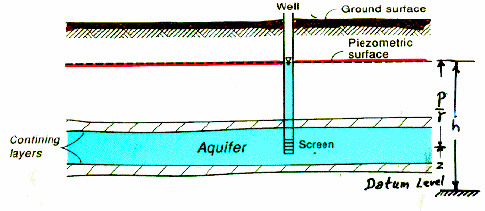
\includegraphics[width=0.99\linewidth]{conaq.jpg}

  Řez zvodní s volnou hladinou (výška zavodněné části je rovna rozdílu mezi piezometrickou výškou a dolní nepropustnou vrstvou).

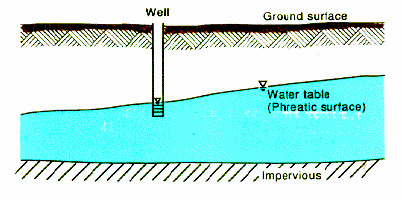
\includegraphics[width=0.99\linewidth]{phraq.jpg}
  
\end{minipage}


Zapište pomocí vhodných veličin, operátorů a rovnic následující vztahy, zákony nebo pozorování,
odpovězte na otázky a splňte úkoly.
\begin{enumerate}[A)]
\item \textit{Darcyho zákon vyjádřený pro celou zvodeň (od povrchu k nepropustnému podloží)}:
  Průtok na jednotku šířky, $\vec q$, má v izotropním prostředí směr
  maximálního poklesu piezometrické hladiny a co do velikosti je
  úměrný tomuto poklesu. Koeficient úměrnosti se nazývá koeficient
  průtočnosti nebo transmisivita a označuje se $T$.
\item Jak zpravidla modifikujeme předchozí odpověď, pokud zvodeň není
  izotropní a má v různých směrech různé vlastnosti?
\item Často pracujeme s veličinou \textit{filtrační rychlost} $\vec v_f$, která
  udává, jaký objem proteče jednotkovou plochou kolmo na směr proudění
  za jednotku času. Jaký bude vztah mezi $\vec v_f$ a $\vec q$? Uvažujte pouze
  speciální případ, kdy je $\vec v_f$ konstantní v celé tloušťce zvodnělé
  vrstvy $b$. (Tloušťka zvodnělé vrstvy $b$ je u proudění s volnou hladinou rovna vzdálenosti piezometrické hladiny od dolní nepropustné vrstvy a u proudění mezi nepropustnými vrstvami rovna vzdálenosti těchto vrstev.) 
  \stranka
\item \textit{Zákon zachování pro vodu}: Množství vody v daném místě (v metrech krychlových vody na metr čtvereční povrchu zvodně) označte $v$. Rychlost s jakou se kumuluje voda v daném místě v kubických
  metrech (vody) na čtvereční metr (povrchu zvodně) za den, tj. derivace $v$ podle času, je
  součtem
  \begin{itemize}\itemsep 0 pt
  \item vydatnosti zdrojů v tomto místě ($\sigma$, v kubických
    metrech vody na metr čtvereční povrchu zvodně za den, může se jednat například o zasakování srážek) a
  \item rychlosti, s jakou v daném místě klesá tok $\vec q$.
\end{itemize}
  Vyjádřete tento zákon kvantitativně pomocí vhodné rovnice.
\item Objem vody v podzemí souvisí s hladinou podzemní
  vody. \textit{Zásobnost} $S_s$ udává, jaký objem vody se uvolní na
  metru čtverečním povrchu zvodně, pokud se piezometrická hladina
  v tomto místě sníží o jednotku. U zvodně s volnou hladinou je tato
  veličina dána zejména pórovitostí půdy nebo horniny, u zvodně s
  napjatou hladinou souvisí se stlačitelností a proto je v tomto
  případě zásobnost velmi malá. Jaká je jednotka takto definované
  zásobnosti a jak souvisí rychlost s jakou roste objem vody v daném
  místě zvodně s rychlostí, s jakou roste piezometrická hladina
  v tomto místě?
\item Předchozí odpovědi spojte do rovnice 
  podzemní vody v anizotropním prostředí.
\end{enumerate}

\textit{Podle Jacob Bear, Modeling Groundwater Flow and Pollution a Charles Fitts, Groundwater Science.}

\reseni

\begin{enumerate}[A)]
\item $\vec q=-T \nabla h$ kde $T$ je koeficient průtočnosti a $-\nabla h$
  je vektor mířící ve směru nejrychlejšího poklesu piezometrické
  hladiny $h$ a vyjadřující rychlost tohoto poklesu.
\item $T$ je  $2\times 2$ matice
\item $\vec q=b\vec v_f$
\item $\frac{\partial v}{\partial t}=\sigma-\mathop{\mathrm{div}}\vec q$
\item Zásobnost je vlastně změna objemu (vody) na jednotkovou plochu
  (zvodně) vyvolaná  jednotkovou změnou délky (změna piezometrické hladiny),
  tj. derivace $v$ podle $h$ a jednotkově vychází bez rozměru. Platí tedy
  \begin{equation*}
    \derivace vh=S_s \end{equation*}
  kde $v$ je objem vody na
  metr čtvereční povrchu zvodně v daném místě. Po vynásobení rychlostí s jakou se
  mění piezometrická výška dostáváme
  \begin{equation*}
    \derivace vh \derivace ht=S_s\derivace ht
  \end{equation*}
   a po využití derivace složené funkce
  \begin{equation*}
    \derivace vt=S_s\derivace ht.
  \end{equation*}
  Toto se děje v libovolném místě zvodně. Protože $v$ a $h$ jsou i funkcemi proměnných $x$ a $y$ a protože souřadnice $x$ a $y$ jsou nezávislé na čase, stačí pro korektní zápis použít parciální derivace namísto obyčejné derivace, tj.
  \begin{equation*}
       \frac{\partial v}{\partial t} = S_s \frac {\partial h}{\partial t}.
     \end{equation*}
\item
  \begin{equation*}
    S_s\frac{\partial h}{\partial t}=\sigma - \mathop{\mathrm{div}} \left(-T\nabla h\right)
  \end{equation*}
  tj. 
  \begin{equation*}
    S_s\frac{\partial h}{\partial t}=\sigma + \mathop{\mathrm{div}} \left(T\nabla h\right)
  \end{equation*}

\end{enumerate}
\konec
\stranka

\subsection{Rovinné proudění podzemní vody podruhé}

Prozkoumáme podruhé rovinné proudění, kterému jsme se věnovali v
příkladě \ref{pokles}.

\begin{enumerate}[A)]
\item Rovnici podzemní vody ve 2D rozepište do složek. Uvažujte pro jednoduchost izotropní prostředí (transmisivita je skalární veličina, tj. ne matice a voda teče ve směru spádu piezometrické hladiny).
\item Napište rovnici z předchozího bodu pro \textit{stacionární} případ \textit{bez zdrojů} a pro případ, že funkce $h$ nezávisí na $y$. Uvažujte homogenní prostředí a zvodeň s volnou hladinou a vodorovnou dolní nepropustnou vrstvou, kde volíme nulovou hladinu $h$ (tj. transmisivita je tvaru $$T=kh,$$ kde $k$ je reálné číslo, ne funkce proměnných $x$ a $y$)
\item Ukážeme, že rovnice se dá vyřešit i bez znalosti řešení diferenciálních rovnic. Upravte vztah z předchozího bodu použitím zřejmé identity
  $(h^2)'=2 h h'$
  pro $h$ jako funkci proměnné  $x$, kde čárka značí derivaci podle $x$. Výsledkem bude podmínka, kterou musí splňovat funkce $h^2$ a odsud již najdete hledanou křivku snížení piezometrické hladiny. (Pokud je $h$ závislé jenom na $x$, plocha ohraničující zvodnělou vrstvu se z bočního pohledu promítne do křivky.)
\end{enumerate}


\reseni
\begin{enumerate}[A)]
\item $$S_s\frac{\partial h}{\partial t}=\sigma + \frac{\partial }{\partial x}\left (T \frac{\partial h}{\partial x} \right)
  +
  \frac{\partial }{\partial y}\left (T \frac{\partial h}{\partial y} \right)
  $$
\item Protože máme uvažovat stacionární případ, funkce $h$ nezávisí na $t$. Podle předpokladu $h$ nemá záviset ani na $y$. Proto platí $h=h(x)$, tj. derivace $h$ podle $t$ a podle $y$ jsou nulové.
  Protože nemáme uvažovat zdroje, je $\sigma$ také nulové. Protože máme uvažovat homogenní případ a $T=kh$, můžeme konstantu $k$ a dát před derivaci.  Rovnice má tvar
  $$0=k\frac{\partial }{\partial x}\left ( h\frac{\partial h}{\partial x} \right)
  $$
  anebo (využitím stručnějšího zápisu pro derivace funkce jedné proměnné)
  $$0=k(h h')'.$$
\item Dostáváme $h h' = \frac12 (h^2)'$ a po dosazení
$$0=k\left(\frac 12 (h^2)'\right )'.$$ Po vydělení rovnice konstantou $k$ a vynásobení faktorem $2$ dostaneme 
  $$0=(h^2)''.$$
  Druhá derivace funkce $h^2$ tedy musí být nula. Proto je $h^2$ nutně lineární funkcí proměnné $x$, tj. existují konstanty $C_1$ a $C_2$ tak, že platí $$h^2=C_1x+C_2.$$
  Křivka odpovídá výsledku příkladu  \ref{pokles}, kde je
  $$h^2=\frac{-2q}k x + \text{const.}$$
\end{enumerate}
\konec


\section{Diferenciální rovnice II}

\section{Autonomní systémy}

\section{Diferenciální rovnice druhého řádu}

\section{Více integrálů}

\section{Více diferenciálních rovnic}

\section{Shrnutí}






